\documentclass[11pt,english]{article}

\usepackage{amssymb,amsfonts,amsmath}
\usepackage{mathtools}
\usepackage{setspace}
\usepackage{sourceserifpro}
\usepackage[T1]{fontenc}
\usepackage{graphicx}
\usepackage[left=1in,right=1in,top=1in,bottom=1in]{geometry}
\usepackage[authoryear]{natbib}
\usepackage{enumerate}
\usepackage{hyperref}
\usepackage{booktabs}
\usepackage{pdflscape}
\usepackage{tabularx}
\usepackage{longtable}
\usepackage{epstopdf}
\usepackage[utf8]{inputenc}
\usepackage{multirow}
\usepackage{subcaption}
\usepackage[flushleft]{threeparttable}

\usepackage{tikz}
\usetikzlibrary{positioning}
\usepackage{subcaption}
\usepackage[shortlabels]{enumitem}


\usepackage{bbm}
\usepackage{forest}
\usepackage{float}
\usepackage{rotating}

\usepackage{algorithm}
\usepackage{algpseudocode}
%\newtheorem{assumption}[theorem]{Assumption}

\hypersetup{
colorlinks=true,
linkcolor=blue,
filecolor=magenta,
urlcolor=blue,
citecolor=blue,
}
\urlstyle{same}
\def\sym#1{\ifmmode^{#1}\else\(^{#1}\)\fi}
\newcommand*\file[1]{\href{run:#1.pdf}{#1}}
\urlstyle{same}
\newtheorem{theorem}{Theorem}[section]
\newtheorem{lemma}[theorem]{Lemma}
\newtheorem{proposition}[theorem]{Proposition}
\newtheorem{definition}[theorem]{Definition}
\newtheorem{assumption}[theorem]{Assumption}
\newtheorem{corollary}[theorem]{Corollary}
\newenvironment{proof}[1][Proof]{\begin{trivlist}
\item[\hskip \labelsep {\bfseries #1}]}{\end{trivlist}}

\begin{document}
\setstretch{1.5}
\begin{titlepage}
\title{Behavioral Machine Learning? \\ Computer Predictions of Corporate Earnings also Overreact}
\author{Murray Z. Frank, Jing Gao, and Keer Yang\thanks{Frank is from University of Minnesota, Minneapolis, MN, E-mail: murra280@umn.edu. Gao is from University of Minnesota, Minneapolis, MN, E-mail: gao00268@umn.edu. Yang is from University of California at Davis, Davis, CA, E-mail: kkeyang@ucdavis.edu. None of the authors have any relevant or material financial interests related to the research described in this paper. We are grateful for helpful comments from Jiangze Bian, Nirmol Das, Ke Tang, Colin Ward, Andy Winton, Moto Yogo and seminar participants at the University of Minnesota, 2023 JFDS Conference, 2023 ABFER, HKUST, and SUSTech Research Conference on Capital Market Research in the Era of AI, 2023 Cardiff Fintech Conference, 2023 FMA, 2023 KAIST AI Social Science BootCamp, and UC Davis Finance Day. We are responsible for all errors.}}

\date{\today}
\maketitle
\thispagestyle{empty}

\begin{abstract}
\begin{singlespace}
Machine learning algorithms are known to outperform human analysts in predicting corporate earnings, leading to their rapid adoption. However, we show that leading methods (XGBoost, neural nets, ChatGPT) systematically overreact to news. The overreaction is primarily due to biases in the training data and we show that it cannot be eliminated without compromising accuracy. Analysts with machine learning training overreact much less than do traditional analysts. We provide a model showing that there is a tradeoff between predictive power and rational behavior. Our findings suggest that AI tools reduce but do not eliminate behavioral biases in financial markets. 

\end{singlespace}
\end{abstract}

JEL Classification: G17, G32, G40

Key Words: Overreaction, behavioral finance, machine learning 

\end{titlepage}

%\clearpage
%\tableofcontents
%\listoftables

\DeclareGraphicsExtensions{.pdf,.png,.gif,.jpg}
\newpage

\section{Introduction}
A basic promise of the machine learning revolution is that algorithms being free from human psychological biases and human emotions, should produce higher quality and more rational predictions  than humans produce. \citet{van2022man} and \citet{cao2021man} show that in fact machine learning models can outperform human analysts in predicting corporate earnings by up to 15\%. Due to their predictive advantage it is no surprise that we have been seeing widespread adoption of algorithmic forecasting by stock analysts. But better average performance, is not the same thing as actually being rational. Our question is simple. Do machine learning predictions actually satisfy rational expectations as commonly defined, under standard tests \citep{bordalo2021real,bordalo2022overreaction}? It appears that many people implicitly assume that the answer is `yes'. But, is it?

In this paper we test the rationality of corporate earnings forecasts produced both by machine algorithms and by professional human stock analysts. The main data are earnings forecasts from IBES (1994-2018), firm financial data from Compustat, stock returns from CRSP, macroeconomic data from the Philadelphia Fed. We also manually collected analyst background educational information from LinkedIn and FINRA. The data are used to train various machine learning models, and those models are used to predict corporate earnings. The predictions are tested directly for rationality. The predictions are also compared to human stock analyst predictions. 

To help clarify the forces at work, a new model is presented. It is a modified version of \citet{begenau2018big}. There is a  firm that makes investment decisions and issues equity. Investors look at analyts predictions prior to deciding their investments in corporate equity. By altering the mix of rational and behavioral analysts in the model and simulating, the model is used to quantify the impact of biases in the underlying data on the predictions generated from that data. In our model there are two sources of bias. First, the training data reflects a mixture of rational and overreacting agents. Second, standard regularization methods systematically underweight certain signals. In the simulations the degree of behavioral bias in training data is controlled. It turns out that biases in the training data is likely a primary source of observed machine overreaction.

Contrary to the common presumption, predictions generated by the algorithms reject the rationality hypothesis. Much like humans, the computers generate predictions that overreact to news. This is true for a range of algorithms including gradient boosted regression trees (XGBoost), neural networks, and even large language models (ChatGPT). The machine predictions  overreact less strongly than do human analysts. But significant bias persists. There is overreaction to both firm-specific news, and to market-wide information. So it does not seem to be limited to just a particular type of information.

Our findings have potentially useful real-world implications. We document that analysts with technical backgrounds who were better positioned to adopt ML tools after 2013 had weaker overreaction than did traditional analysts. Getting rid of the overreaction is potentially harmful at least in the cases studies here. Algorithmic adjustments can be used to reduce overreaction. But this comes at the cost of decreased predictive accuracy. So there is a fundamental trade-off between forecast accuracy in the sense of mean squared error, and bias in the sense of overreaction to news. 

In the behavioral economics and finance literature \citep{bordalo2020overreaction} it is commonly thought that observed failures of rationality documented in human decisions are due to psychology and the deep structure of the human brain. But, of course our machine algorithms have no human brains. Yet they exhibit overreactions much like humans. Thus the standard behavioral explanation might not be correctly identifying the actual source of the failures of rationality. Biases in the underlying data appear to be important, with or without humans making the predictions. 

Our paper makes several novel contributions. First, machine learning predictions are shown to exhibit overreaction  to news. This challenges the common impression that algorithms are rational since they are not subject to human emotions. Second, a new model is provided to  explain how training data biases can produce overreaction in machine predictions. Third, we offer new evidence showing how machine learning adoption influences analyst forecast quality for analysts with different educational backgrounds. Finally, we have demonstrated that there is a critical trade-off between reducing behavioral bias in the sense of overreaction, and maintaining predictive accuracy when using machine learning generated predictions.


\paragraph{Related Literature}
Our paper connects to and extends four main strands of literature. Start with research on machine learning applications in financial prediction. Studies by  \citet{van2022man} and \citet{cao2021man} document ML's superior predictive power compared to human analysts in various settings. We show that this advantage comes with previously undocumented behavioral biases. Using gradient boosting regression trees, we find accuracy improvements similar to \citet{van2022man}. They are as dramatic as in \citet{cao2021man}. We are the first to document systematic overreaction in ML-generated corporate earnings forecasts. This shows a crucial limitation in the performance of these models.

There is a literature that focuses on understanding of belief formation and expectations in financial markets. \citet{bianchi2022belief} uses ML as a benchmark to study human analyst biases. We go further by analyzing potential biases within ML predictions themselves. We show that ML models exhibit overreaction in firm-level predictions, despite showing less bias in aggregate forecasts. Thus we offer a new insight into how algorithmic predictions might vary across different settings. Our examination of the distinction between firm-specific and aggregate prediction behavior represents a potentially important contribution to the understanding of ML applications in finance.

We extend the literature on algorithmic bias (\citet{danks2017algorithmic}, \citet{mehrabi2021survey}, \citet{baeza2018bias}, \citet{das2023algorithmic}) to the domain of financial forecasting. Previous work by \citet{greenwald2024regulatory} has documented algorithmic bias in lending decisions. Our study is the first to show how such biases can emerge in earnings predictions and affect real investment decisions. By demonstrating that analysts who adopt ML tools show reduced but persistent overreaction, we provide novel evidence of the way in which algorithmic biases translate into real economic outcomes.

There is an emerging intersection between behavioral economics and machine learning. \citet{caplin2025modeling} show alignment between ML predictions and capacity constrained learning models. We provide empirical evidence that ML algorithms exhibit systematic behavioral biases similar to humans. Our evidence suggests that even sophisticated ML models may be subject to cognitive limitations analogous to human decision-makers. This raises issues about the algorithms themselves. It also raises concerns about the standard interpretation of overreactions in the behavioral literature \citep{bordalo2022overreaction}. Contrary to the usual presumption, human psychology might not be responsible for the evidence provided in that literature. 

The rest of the paper is organized as follows. Section \ref{sec:Data} describes the sources of information fed into the prediction algorithms. Empirical strategies are explained in Section \ref{sec:methods}, along with a test for overreaction. Section \ref{sec:MainResults} presents the key test results. Section \ref{sec:why} examines why machine learning predictions overreact. Section \ref{sec:model} introduces a formal model and a simulation exercise to help interpret the evidence. Section \ref{sec:chatgpt} presents the first implication of our results in a generative AI setting. Section \ref{sec:analysts} discusses the second implication in the context of stock analysts. The conclusion is in Section \ref{sec:conclusion}.


%%%%%%%%%%%%%%%%%%%%%%%%%%%%%%%%%%%%%%%%%%%%%%%%%%%%
\section{Data}
\label{sec:Data}
Our main empirical analysis uses four data sources: (1) Firm earnings forecasts (EPS) by equity analysts, sourced from IBES; (2) Firm financial data from Compustat, and stock return data from the Center for Research in Security Prices (CRSP); (3) Macro time series downloaded from Federal Reserve Bank of Philadelphia real time data; and (4) Manually collected background information on equity analysts obtained from LinkedIn and cross-references with FINRA brokercheck. 

Our sample begins from 1994 and ends in 2018 to exclude the Covid period. As a result we do not cover the ChatGPT era that began roughly near the end of 2022, i.e. post Covid. Our sample period is sufficiently long to study the real impact of analysts before the widespread adoption of ChatGPT and after it became widely known. 

\subsection{Earnings Forecasts}
We use annual earnings data from I/B/E/S as our forecasts. We obtain actual earnings per share (EPS) from the I/B/E/S Actual files. We do not use the earnings data from Compustat due to its utilization of different accounting methods for measuring actual earnings. For prediction purposes, we use the raw EPS data from I/B/E/S.\footnote{Although the total number of shares may vary across years, we do not adjust for it when making the predictions. The results are similar when we use earnings per total assets instead of earnings per share as a forecast. We adjust for changes in the number of shares when calculating forecasting errors.} 

We examine analysts' earnings forecasts instead of price forecasts to be consistent with empirical tests in the behavioral finance literature, which test analysts' overreacting earning forecasts.

%Our objective is to compare analysts' forecasts with machine learning predictions. To achieve this, we employ the realized earnings from the I/B/E/S database as a training sample for the machine learning model to forecast earnings.

\subsection{Forecasting Variables used to Forecast Earnings}
We utilize publicly available signals as forecasting variables to predict earnings. First, we use financial ratios downloaded from the Wharton Research Data Service (WRDS) Financial Ratio suites. The detailed definition of financial ratios is provided in Appendix Table. We exclude financial ratios with a large number of missing observations, resulting in a total of 65 firm characteristics used as predictors. For other variables, we replace the missing values with the industry average. 
%We exclude PEG\_trailing, divyield, pe\_op\_basic, and pe\_op\_dil due to a large number of missing observations, resulting in a total of 65 firm characteristics used as predictors. For other variables, we replace the missing values with the industry average.

We then include last year's annual earnings per share and the quarterly earnings per share from the last three quarters obtained from the I/B/E/S database. We also incorporate the analysts' median forecast of EPS as forecasting variables. The details on how to construct analysts' median forecast of EPS will be discussed in the next subsection. To capture the most current market conditions, we include the stock price and monthly stock return into the forecasting variables for the respective forecasting month.

We use macroeconomic variables as forecasting variables. We obtain the data from the Federal Reserve Bank of Philadelphia's real-time dataset. We use the following variables: Real GDP, Real GDP Growth, Real Total Personal Consumption Expenditures, Real Total Personal Consumption Expenditures Growth, Total Industrial Production, and Unemployment Rate.

In addition to the main prediction model, certain prediction models incorporate items from firms' balance sheets as forecasting variables. These signals may or may not correlate with the WRDS Financial Ratio. The capability of machine learning for variable selection enables us to include those variables, even if they yield similar signals.

\subsection{Analysts' Earnings Forecasts}

The IBES database provides micro-level data on firm-level forecasts made by equity analysts. These analysts make monthly forecasts before the end of the fiscal year. We use equity analysts' forecasts of firms' annual earnings per share (EPS) with a forecasting horizon ranging from 12 to 23 months. The forecasting horizon is the difference in months, between the fiscal year end month of the realized annual EPS to be predicted, and the month when the analyst made the forecast. For each firm and each month, we calculate the median value of the forecasts to determine the median consensus forecast for next year's annual EPS.

\subsection{Analysts' Technical Backgrounds}
A key concern is the distinction between analysts with different education and technical skills. The data we need is not provided by IBES. We manually collect the technical backgrounds of analysts using their LinkedIn information. Our goal is to measure analysts' statistical tools, and therefore their ability and probability of incorporating machine learning in their EPS forecasts. Here the focus is on the analysts and their backgrounds.

\begin{center}
******************************************* \\
\textbf{Figure \ref{fig:LinkedIn} about here}. \\
*******************************************
\end{center}

To identify analysts' identity and educational background information, we use analysts who gave at least one earnings recommendation in 2018. We cross-check their affiliations on FINRA's brokercheck website and LinkedIn to maximize the likelihood of an accurate manual matching. In total, we successfully linked 858 analysts to their LinkedIn profiles.

To identify analysts' technical backgrounds start with self-reported technical skills, including machine learning, artificial intelligence, and advanced statistics. It should be noted that we do not use `quantitative modelling' as a keyword since it might refer to a much wider range to prediction methods. Figure \ref{fig:LinkedIn} gives an example of a technical analysts' LinkedIn page.

We use their higher education background to identify whether analysts have technical skills or not. We manually check the curriculum for each major and identify the majors in Table \ref{tab:majors} as technical majors. These majors are mostly STEM majors, but there are some discrepancies. For example, we do not find advanced statistical courses in the biology major's curriculum. So analysts with a general biology education are not generally included. However, if an analyst earns a degree in Computational Biology, we find that advanced statistical tools are required. Therefore, we label these analysts as technical analysts.\footnote{Our focus is different from \citet{babina2021artificial}, which focuses on AI-related skills instead of statistical skills. We aim to measure analysts' ability to understand and use advanced statistics and the probability of using them. Therefore, we do not only focus on AI-related skills.}

In total, we identified 173 analysts with a technical education background. We then distinguish our IBES sample to analysts whom we categorized as technical vs. non-technical. For each firm in each month, we calculated the median consensus forecast by technical analysts $F_t^{T} Y_{i,t+1}$ and non-technical analysts $F_t^{NT} Y_{i,t+1}$ separately.

To conduct the overreaction test, in each fiscal year $t+1$, we took the average of the 12 median consensus forecasts made during fiscal year $t+1$. Starting in 1994 and going to 2018 we have 14,901 firm-year observations for forecasts made by technical analysts and 36155 firm-year observations for forecasts made by non-technical analysts. It should be kept in mind that technical analysts and non-technical analysts may cover different stocks, and this may affect certain comparisons.


%%%%%%%%%%%%%%%%%%%%%%%%%%%%%%%%%%%%%%%%%%%%%%%%%%%%

\section{Empirical Methods}
\label{sec:methods}

Many models and empirical frameworks can be used to evaluate predictions. We report results for  linear regressions because they have been in use for a long time and are familiar. Similar results are obtained by using \citet{fama1973risk} regressions, but to save space we do not report those results in detail. We report results for Gradient Boosting since is a particularly successful and widely used Machine Learning method. We use two high profile software library implementations of the method and obtain very similar results from each.

\subsection{Linear Regressions}
A particularly simple and widely used approach to evaluate the forecasts of Earnings Per Share is to use a linear regression. We use average mean squared errors $MSE$ to measure the predictive performance of each model.
\begin{equation}
	MSE  = \frac{\sum_i(y_{i,t+1} - F_t y_{i,t+1} )^2}{N}
\end{equation}


\subsection{Using ML to Make Predictions}
The machine learning predictions mimics the forecasts by equity analysts. Equity analysts made forecasts monthly on the annual EPS of the firm. For EPS of firm i in each fiscal year, we ask the machine learning model to make predictions each month from 12 to 23 months prior to the end month of the fiscal year, using the most updated information available during the month. We use observations in the past 5 years to train the model. Suppose our forecast horizon is $h$ month, $h = 12, 13.., 23$. We made forecast using information available in year $t$ at year-month $m$, denote as $X_{i,m}$. Because forecast horizon is $h$, we want to predict EPS of firm $i$ at year-month $m+h$, denoted as $y_{i,m+h}$. In this case, $m+h$ should be firm i's fiscal year end month. If the year-month $m+h$ is not firm's fiscal year end month, we do not make predictions. The model is trained using observations from $t-5$ to $t-1$.

The information set $X_{i,m}$ of firm $i$ at year-month $m$ includes: (1) last annual EPS, the last three quarters' quarterly EPS; (2) financial ratios from the Financial Ratios Suite by WRDS, stock price and monthly return, which provide firm-month level information that is available at year-month $m$; (3) macro variables calculated using Federal Reserve Bank of Philadelphia real-time data; and (4) the median consensus forecast of analysts at each firm-month. We also use the monthly median consensus forecast of analysts to incorporate the idea of the importance of analysts' private information. For each investment horizon $h$ at each month-year $m$ (denote $t$ as the calendar year of the month-year $m$), we use a training sample consisting of five-year observations prior to the forecast date year $t$. The training sample includes the ${X_{i,\tau}, y_{i,\tau+h}}$ where $\tau$ are within year $t-5$ and $t-1$, and $y_{i,\tau+h}$ is publicly available by the end of $t-1$.\footnote{This restriction is stricter than $\tau+h \leq m$ because earnings are usually reported with a lag.} We retrain the model each year to make forecasts for the following year.

If we are given the information set $X_{i,m}$ in year $t$ at year-month $m$ and we want to forecast the annual EPS realization in the fiscal-year end month $m+h$, we can make predictions based on the following model:
\begin{equation}
    F_{m} y_{i,m+h} = f_y^h(X_{i,m})
\end{equation}
where $f_y^h$ is trained using the past 5-year observations. $f_{y}^h X_{i,m}$ is the machine learning model's year-month $m$ forecast for firm $i$'s annual EPS realization at the fiscal year end month $m+h$. Similar to analysts, the machine learning model could make forecast at any month before fiscal year end month.

\subsection{Gradient boosting regression tree}
The machine learning algorithm we used is gradient boosting regression tree model. Gradient boosting regression trees are a particularly prominent and
empirically successful prediction method used in many applications. It starts
with regression trees and then refines them iteratively by focusing on the
errors in the previous iteration. This idea of refinement by focusing on error
correction is known as boosting. Gradually an entire forest of trees is
constructed. Then an average across the set of trees is used as the model's
prediction.


% \begin{figure} 
%     \caption{Tree Example}
%     \label{fig:TreeExample}
%     \centering
%     \begin{forest}
% 	for tree={l sep+=.8cm,s sep+=.5cm,shape=rectangle, rounded corners,
% 		draw, align=center,
% 		top color=white, bottom color=white}
% 	[{ $\pi_t < 0.5$}
% 	[ {ln $B_t/M_t < 1$} , edge label={node[midway,left]{True} }
% 	[{$\pi_{t+1} = 0.1$ }, edge label={node[midway,left]{True}}  ]
% 	[{$\pi_{t+1} = 0.5$ }, edge label={node[midway,right]{False} }  ]
% 	]
% 	[{$\pi_{t+1} = 0.8$ }, edge label={node[midway,right]{False} }]
% 	]
%     \end{forest}
% \end{figure}


Gradient boosting is the most widely adopted version of boosted forests. It
starts by estimating decision trees with fixed shallow depth. Then it computes
the residuals for the trees. At the next iteration more weight is devoted to
the cases in which the model fit poorly. In the end an ensemble of trees are
used to `vote' on the appropriate results. This generally reduces the bias in a
simple tree model while maintaining the low variance. The main drawback
relative to a simple tree is that forests
do not have such simple depictions that show how each variable affects the
final result.

There are three important hyper-parameters in gradient boosting: the depth of the
tree $d$ (max$\_$depth), the number of trees in the forest $M$ (n$\_$%
estimators), and learning rate $\gamma$ (learning$\_$rate). The default
parameters we use have the following values: depth of the tree is $2$, number of
trees in the forest is $50$, and learning rate is $0.1$. This set of hyper-parameters are obtained through cross-validation method using sample before 1994. We have
systematically carried out the analysis with the hyper-parameters optimized using cross-validation. The hyper-parameters were chosen to optimize the out-of-sample mean squared errors before 1994.  Except where noted, the Tables use the default hyper-parameters.

A more formal representation can be found in Section \ref{sec:ml_parameters} when we examine the variation in model hyper-parameters. Gradient boosting estimation was done using the software
GradientBoostingRegressor from
\url{https://scikit-learn.org/stable/modules/ensemble.html}, and also using XGBoost from
\citet{chen2016xgboost}. The results for the two implementations of gradient boosting are very similar. The reported results in the Tables use the algorithm GradientBoostingRegressor from \url{https://scikit-learn.org/stable/}.


\subsection{Testing for Overreaction}\label{sec:overreaction}
We follow the framework proposed by \citet{bordalo2021real} to test for overreaction in analysts' and machine forecasts. We start with the monthly consensus forecasts made by analysts and the monthly forecasts made by machine learning model. For each EPS of firm $i$ at fiscal year $t+1$, we have machine learning forecasts and consensus analysts forecasts made 12 to 23 months prior to the fiscal year end month. We take the average of the 12 machine learning forecasts. This is the average forecasts made during fiscal year $t$ on the EPS of firm at fiscal year $t+1$, denoted as $F_t y_{t+1}$.

We merge the firm-year level forecasts to standard firm financial data from COMPUSTAT. We then convert the per share forecasting error to per total assets forecasting error, by multiplying firm's total number of shares and divided by total assets. Earnings per unit of total assets are denoted as $y_{i,t}$.  The results are similar when we instead scaled by total capital stock. All firm level variables are scaled by total assets. We further restrict our sample to forecast made from 1994 to 2018, with at least one analyst forecast, resulting in $54534$ firm-year observations.

To test for overreaction, following \citet{bordalo2021real}, we run the following regression.
\begin{equation}
    y_{i,t+1} - F_{t} y_{i,t+1} = \beta x_{i,t} + \lambda_t + \mu_i + \varepsilon_{i,t}
\end{equation}

The dependent variable is next year's forecast errors, which is defined as realized earnings ($y_{i,t+1}$) minus predicted earnings ($F_{t} y_{i,t+1}$). We regress the forecast errors on current-year firm investments ($x_{i,t}$), controlling for time and firm fixed effects. If the forecast falls within rational expectations, the forecast errors should be unpredictable based on any information available at the time of the forecast. If the forecast overreacts, which means that the forecast is overly optimistic during good times and pessimistic during bad times, then the forecast will be too high during good times and too low during bad times. As a result, the forecast errors will be negatively correlated with the firm's current fundamentals, such as the investment rate. The coefficient $\beta$ before $x_{i,t}$ captures the extent of overreaction in the forecast $F_{t} y_{i,t+1}$.\footnote{A formal derivation of the \citet{bordalo2021diagnostic} test is provided in Appendix \ref{sec:appframework}.}

To examine the magnitude of overreaction, we also compare the difference in overreaction coefficients ($\beta$) using different forecast models. We use seemingly unrelated regressions to compare the regression coefficients using forecasting errors from different forecast models. We report $\chi^2$ statistics and p-values of Wald tests calculated using covariance estimated from the seemingly unrelated regressions. Because any contamination from measurement errors and fixed effects is the same when we use different forecast errors, we can directly compare the coefficients $\beta$. A lower $\beta$ indicates a lower overreaction coefficient.



%%%%%%%%%%%%%%%%%%%%%%%%%%%%%%%%%%%%%%%%%%%%%%%%%%%%
\section{Empirical Results}
\label{sec:MainResults}
In this section, we first analyze the predictability of machine learning models versus analysts' forecasts by comparing the mean squared errors of each forecasting method. Then, we examine whether the machine learning algorithm exhibits overreacting behavior. We find that machine learning forecasts experience similar overreacting behavior, but with a smaller magnitude. We explore potential explanations by comparing machine learning models with different forecasting variables and regularization parameters. Finally, we examine whether similar overreacting behavior also exists when we use linear regression models.

\subsection{Prediction MSE}
This section provides an overall evidence on the predictability of firm earnings. Table \ref{tab:sumstat} presents evidence on the efficacy of gradient boosting methods, analyst forecasts, and linear regression models. 

\begin{center}
******************************************* \\
\textbf{Table \ref{tab:sumstat} about here}. \\
*******************************************
\end{center}

The first column indicates the variables used as forecasting variables. The set of factors labeled `All' is our benchmark set of factors used for prediction, described in Section \ref{sec:Data}. We also use different sets of factors in the model. The second column represents the learning rate hyper-parameter we use to control for over-fitting in gradient boosting tree models; the default number is $0.1$. The third column represents the mean squared error of forecasts of firm annual EPS. The last column indicates the ratio of the MSE of the analyst's forecast and the forecast model used in that row. A ratio larger than one indicates that the model in the row performs better than the median consensus analyst forecast.


Row (1) of Table \ref{tab:sumstat} presents the prediction results for the median consensus analyst forecast, which serves as our benchmark for mean squared error. The mean squared error of the analyst's forecast is $1.315$.

Row (2) of Table \ref{tab:sumstat} presents the prediction results for gradient boosting using all factors. The model performs relatively well, with an $MSE$ of 1.261. The analyst's forecast has a 4.3\% higher squared forecast error. The results suggest that our machine learning model improves predictability, but not as strongly as in other settings (\citet{cao2021man}). The improvement is similar to the estimation results from \citet{van2022man}.

\citet{cao2021man} argue that human forecasts can complement machine learning forecasts. In the main set of forecasts, we already include the median consensus analyst forecast as a predictor. To examine the importance of the analyst's forecast, we remove it from the factors. When we remove the analyst's forecast as a predictor in row (3), the mean squared errors drop to 1.506, which is much larger than the mean squared error in row (1). The results suggest that when forecasting firm earnings, the analyst's private assessment is extremely valuable. The information generated by analysts cannot be replaced by incorporating a large set of public financial ratios.

In row (4), we extend the set of variables to include all firm balance sheet variables. The mean squared errors are very similar to row (2), suggesting that the financial variables we used in the main forecasting set have already captured the firm heterogeneity in explaining earnings.

Rows (5) to (7) capture the predictability when we use different learning rate parameters. When the learning rate is very small, the model does not fit the training sample enough, which leads to relatively poor out-of-sample performance. As we increase the learning rate, the model's performance improves. However, row (7) shows that if the learning rate is too large, the model runs the risk of over-fitting the historical information, leading to a drop in prediction performance.


\begin{center}
******************************************* \\
\textbf{Figure \ref{fig:MSE} about here}. \\
*******************************************
\end{center}

We also examine the time-series variations in the relative strength between human analysts and machine learning models. Figure \ref{fig:MSE} shows the ratio of mean squared errors of human forecasts and machine forecasts at different years. A ratio smaller than one suggests that humans beat the machines in that year. From 1994 to 2018, we observed 10 years where humans beat the machines, including 1994, 2003, 2004, 2005, 2009, 2010, 2011, 2012, 2013, and 2017. One possible explanation for humans beating the machines is that the training samples experienced negative shocks and were, therefore, less useful for future earnings predictions. The annual SP500 return in 2000, 2001, and 2022 were -10.1\%, -13.0\%, and 23.4\%, respectively. The annual percentage change of the SP500 index in 2008 was -38.5\%, while in 2015 was -0.73\%. When we include those observations in our 5-year training sample, we find that humans beat the machines.

The results are similar if we use the last three years' observations to train the model, but on average we get a lower decrease in MSE if we use only three years' observations. We also tried to include more years during recessions, as \citet{cao2021man} suggested, and found that the results are similar, with still lower increases in average mean squared errors.

To understand the prediction errors it is important to have a basic sense of the underlying dynamics. Accordingly we estimated AR-1 models for each firm. Figure \ref{fig:autocorrelation} shows that for most firms there is a fairly strong first order autocorrelation. The typical coefficient is well above $0.5$. So earnings per share are strongly autocorrelated for a typical firm.  

\begin{center}
******************************************* \\
\textbf{Figure \ref{fig:autocorrelation} about here}. \\
*******************************************
\end{center}


\subsection{Machines Do Overreact}
In this section, we follow the empirical strategy defined in Section \ref{sec:overreaction}. The key question is whether the ML generated forecasts exhibit similar overreaction behavior to that found for human reported forecasts.

\citet{bordalo2021real} run linear regressions in which the dependent variable
is the error at date $t+1$ of stock analyst predictions from IBES. The
independent variables are date $t$ values of the forecast, profit, investment,
or debt issuance. In each of these regressions firm and year fixed effects are
included. According to \citet{bordalo2021real} under rational expectations the
slope coefficients should be zero. Under diagnostic expectations the slope
coefficients should be negative. That is because of beliefs that overreact both
to good and to bad news. \citet{bordalo2021real} use linear regressions with
fixed effects to carry out this test. 

\begin{center}
******************************************* \\
\textbf{Table \ref{tab:over_main} about here}. \\
*******************************************
\end{center}


We follow \citet{bordalo2021real} in Table \ref{tab:over_main}. %We also add columns (1) and (2) that use the prediction error from analysts.
Columns (1) and (2) confirm the widely documented empirical findings that human forecasts exhibit overreaction behavior. In Column (2), the regression coefficient is $-0.142$, indicating that a one standard deviation increase in investment $(0.061)$ leads to an 8\% higher disappointment in earnings next year $(0.061 * 0.142 / 0.109)$. Columns (3) and (4) perform the same regressions as Columns (1) and (2), but using machine learning predictions instead of human forecasts. The magnitude of the regressions is reduced compared to Columns (1) and (2), but the results in all columns (1) to (4) are negative and statistically significant.

To address concerns about downward dynamic panel bias due to the inclusion of firm fixed effects, we provide GMM estimations in Appendix Table \ref{tab:over_gmm}. The GMM results give us a larger regression coefficient of $0.472$. Both gradient boosting and analyst forecasts exhibit overreacting behavior even when we correct for downward dynamic panel bias. The magnitude is comparable to the coefficient of $0.887$ in \citet{bordalo2021real}. The difference in magnitude could result from different sample firms.

To ensure that our results are not driven by a specific set of predictors used in the model, we compare the differences in overreaction coefficients ($\beta$) across different forecasting models. We use seemingly unrelated regressions to compare the regression coefficients estimated using forecasting errors from different forecast models. We report $\chi^2$ statistics and p-values of Wald tests calculated using the covariance estimated from the seemingly unrelated regressions. Since any contamination from measurement errors and fixed effects is the same when we use different forecast errors, we can directly compare the coefficients $\beta$. A lower $\beta$ indicates a lower overreaction. The mean squared error (MSE) shows the out-of-sample performance of the forecasting models.


\begin{center}
******************************************* \\
\textbf{Table \ref{tab:over_variables} about here}. \\
*******************************************
\end{center}


Table \ref{tab:over_variables} shows the results obtained using different information sets to make predictions. We find that the overreaction bias is not driven by a specific set of predictors used in the model.


\subsection{Overreaction to Aggregate or Firm-Specific Shocks?}
The results from \citet{bianchi2022belief} suggest that macro-economic shocks might affect things differently from firm-specific shocks. So we follow \citet{chen2007price} and decompose machine forecast errors into a market-related variation and a firm-specific variation. We do not examine industry-specific variation because our machine learning models are not trained using industry-specific variables. Consider the following regression:

\begin{equation}
    e_{i,t} = \beta_i + \beta_{i,m} r_{m,t} + \varepsilon_{i,t}
\end{equation}
where $e_{i,t}$ is the forecast error of firm $i$ at year $t$, $r_{m,t}$ is the market forecast error at year $t$, which is the equal-weighted average forecast error at year $t$. We define market-related forecast error as $\hat{\beta}_{i,m} r_{m,t}$ and the firm-specific forecast error as $e_{i,t} - \hat{\beta}_{i,m} r_{m,t}$. In Table \ref{tab:over_decompose}, we regress market-related error and firm-specific error on investment separately.


\begin{center}
******************************************* \\
\textbf{Table \ref{tab:over_decompose} about here}. \\
*******************************************
\end{center}



Columns (1) and (2) show the results for analysts' forecasts. The dependent variable in column (1) is the market-related forecasting errors of human analysts, while column (2) is the firm-specific forecasting errors of human analysts. An increase in investment rate leads to disappointment in earnings forecasts by human analysts next year. In columns (3) and (4), we decompose the forecast errors using the gradient boosting model. The dependent variable in column (3) is the market-related forecasting errors of machine analysts, while column (4) is the firm-specific forecasting errors of machine analysts. The overreaction coefficient in column (3) is $-0.012$, while the overreaction coefficient in column (1) is $-0.040$, suggesting that applying machine learning largely reduces the market-related overreaction. The regression coefficients have similar magnitudes in columns (2) and (4).


\subsection{Overreaction of Other ML Models}
Our analysis is focused on gradient boosting predictions. That is motivated by the wide use and documented success of the algorithm. ``Gradient Tree Boosting or Gradient Boosted Decision Trees (GBDT) is a generalization of boosting to arbitrary differentiable loss functions, see the seminal work of \citet{friedman2001greedy}. GBDT is an accurate and effective off-the-shelf procedure that can be used for both regression and classification problems in a variety of areas...'' \footnote{\url{https://scikit-learn.org/stable/modules/ensemble.html\#gradient-boosting}}.

It is natural to wonder if our overreaction results are specific to that particular algorithm. Below we document that our results are not limited to gradient boosting models. Specifically, we analyze whether predictions made by other commonly used machine learning models also exhibit overreaction bias.

Table \ref{tab:over_ml} presents the forecasts calculated from other machine learning models. We find that random forests and neural network models also generate overreaction bias.

\begin{center}
******************************************* \\
\textbf{Table \ref{tab:over_ml} about here}. \\
*******************************************
\end{center}

\subsection{Linear Regression Models Also Overreact}
We demonstrate that earnings predictions generated by various classes of machine learning models exhibit overreaction bias. These models are inherently complex and designed to capture intricate data structures. Additionally, they incorporate regularization techniques during training, primarily to mitigate overreaction. In contrast, traditional econometric methods, such as ordinary least squares (OLS), possess fundamentally different modeling characteristics. A key question, therefore, is whether predictions from these conventional linear models also exhibit overreaction.

To show this we consider predictions from perhaps the most familiar methods used in finance.  We use linear regression models to forecast EPS. The forecasting procedures strictly follow the procedure used in gradient boosting forecasts. The only difference here is that the function $f_{y}$ used to fit the training sample is a linear regression model. We use the same forecasting variables $\Phi_{i,t}$ as in the gradient boosting model.

\begin{center}
******************************************* \\
\textbf{Table \ref{tab:over_ols} about here}. \\
*******************************************
\end{center}

Table \ref{tab:over_ols} presents the forecasts calculated from linear regression models that use different forecasting variables. In column (1), the forecasting variables included firm characteristics and lagged annual and quarterly earnings. In column (2), the forecasting variables included firm characteristics, analysts' forecasts, and lagged annual and quarterly earnings. In column (3), the variables included firm characteristics, analysts' forecasts, lagged annual and quarterly earnings, and financial statement items.

%Unlike the gradient boosting regression tree model, there is no hyper-parameter governing the level of regularization in OLS. The number of forecasting variables represents the information set used in the model, as well as the potential severity of over-fitting. Table \ref{tab:over_ols} shows that when too many forecasting variables are included in a linear model, the forecast variable has an overreacting coefficient quite similar to that of human analysts. 

Till now, we have observed similar overreaction in both OLS and machine learning predictions, we next discuss the distinct sources of overreaction bias across different predictive models. Furthermore, we demonstrate that the mechanisms underlying overreaction in OLS predictions differ from those in machine learning model predictions. Notably, the OLS model does not exhibit overreaction in a simulated economy where data bias is absent.

Overall, our empirical results suggest that overreaction bias is pervasive when we train the model using firm-level earnings forecasts and firm-level economic ratios. We document consistent overreaction to both firm-level and aggregate-level news. The overreaction results are not limited to a single type of machine learning model; they are observed across multiple machine learning model classes. We also find that overreaction bias is present in predictions generated by the OLS model. Next, we examine the underlying causes of overreaction in both machine learning and OLS predictions. Finally, we conduct empirical tests to validate our hypotheses.

%%%%%%%%%%%%%%%%%%%%%%%%%%%%%%%%%%%%%%%%%%%%%%%%%%%%

\section{Why Does Machine Overreact?}\label{sec:why}
Unlike human, algorithms are not directly grounded in human psychology. Why do we observe overreacting behavioral from algorithm predictions including complex machine learning predictions? 
In this section, we develop hypotheses to explain the overreacting biases in machine learning-based corporate earnings predictions. In our paper, we focus on overreacting bias, a deviation from rational expectations in decision-making. The bias we refer to is a statistical pattern exhibited by the algorithm. We draw from the algorithmic fairness literature to develop hypotheses on the sources of bias.\footnote{The computer science literature has extensively discussed algorithmic fairness. Fairness is defined as "the absence of any prejudice or favoritism toward an individual or group based on their inherent or acquired characteristics" (\citet{mehrabi2021survey}). Unfair algorithms are those that lead to decisions skewed toward a particular group of people.} 

The biases in machine learning predictions can stem from two main sources: biases in the data and biases arising from the algorithm itself. Machine learning models rely on training data to learn patterns and make predictions. Biases in the data can distort what is learned by the machine learning algorithm, leading to biased predictions. Biases stemming from training data have been well-documented in the literature (\cite{buolamwini2018gender}, \citet{suresh2021framework}). Besides, machine learning models usually employ extensive regularization in the training process (bias-variance tradeoff), and many forms of regularization are implicit. Due to this distortion, biases could also arise from the biases generated by the models themselves, even if the training data is not biased \citep{baeza2018bias,li2022dominate}.

To illustrate why machine learning predictions exhibit overreaction bias, we first provide a formal statistical definition of overreaction and then explain the mechanisms through which machine learning predictions can induce such biases.

\subsection{Overreacting Predictions}\label{sec:framework}
In this section, we present a simple framework to clarify the definition of overreaction in the context of machine learning model predictions. We first revisit the definition of overreaction and then introduce a general predictive framework used to explain the overreaction bias of algorithms, without imposing strong parametric assumptions. %We use different symbols to suit the purpose of our illustration.

A forecaster aims to predict future earnings $\varepsilon_i$ of firm $i$ that is currently unobservable to the forecaster. The forecaster observes a signal about future earnings, denoted as $\zeta_i$. This signal provides partial information about the true future earnings $\varepsilon_i$. We assume that both $\zeta_i$ and $\varepsilon_i$ have a mean of zero and a variance of one for simplicity. Additionally, we assume that the signal is positively correlated with true earnings, such that $\text{corr}(\zeta, \varepsilon) = \rho>0$. We define rational and overreacting predictions as follows:

\begin{enumerate}
    \item For a rational model (the predictive model used by rational managers), its prediction, denoted as $x_i$, is given by $x_i = \rho \zeta_i$. That is, when forecasters are rational, their predictions are statistically optimal predictions.
    \item For an overreacting model (the predictive model used by overreacting managers), its prediction is given by $x_i = \kappa \rho \zeta_i$, where $\kappa > 1$. Note that if $\kappa = 1$, then the prediction is rational. 
\end{enumerate}

This definition of overreaction is consistent with the definition we used to conduct the overreaction test in \citet{bordalo2021diagnostic}. We denote the forecast error for firm $i$ as the difference between realized true earnings and predicted earnings, that is, $\varepsilon_i - \kappa \rho \zeta_i$. The relationship between forecasting errors and the signal $\zeta_i$ is given by:

\begin{equation}\label{eq:corr}
    \text{corr}(\varepsilon_i - \kappa \rho \zeta_i , \zeta_i)  = \text{corr}(\varepsilon_i, \zeta_i) - \kappa  \rho = \rho (1 - \kappa).
\end{equation}

If the prediction is rational, the correlation between the forecasting error and the signal is zero. Conversely, if the prediction exhibits overreaction ($\kappa > 1$), the correlation between the forecasting error and the signal is negative.

Next, We discuss how biases in the training data and the algorithm can lead machine learning models to produce predictions that deviate from rational expectations.

\subsection{Bias From the Data}
First, we examine how overreacting data can lead to overreaction bias of machine learning-based predictions. Predictions made by machine learning model trained on biased data could inherit the same bias embedded in the training data. In addition, the biases in the data can be transmitted differently, depending on the predictive models applied to the data. In our paper, we focus on the overreaction bias.

To thoroughly understand this question, we begin by explaining what biased data in the economy means and how algorithms make predictions based on the biased data. Consider the case where managers and analysts in the economy observe public news about future earnings and then make predictions based on it. With these predictions, managers and analysts can make real decisions. However, if predictions are overreacting, agents' decisions will be distorted. For example, managers might make exaggerated hiring or firing decisions, and analysts could overestimate (underestimate) future earnings predictions based on good (bad) news. By contrast, rational analysts and managers would make decisions based on the actual signal without overreacting. One important assumption we make, which is also commonly made in the behavioral economics literature (e.g.,\citet{bordalo2021real}), is that behaviorally biased decisions do not affect the underlying earnings process. This means that next-period earnings are not distorted by biased decisions. 

If economic agents make decisions based on overreacting predictions, the data we collect from this economy will deviate from the data collected from an economy with only rational agents. For example, if a manager has overreacting predictions and make hiring decisions based on these biased predictions, then hiring decisions are distorted. Her hiring decision is still an informative predictor of the firm's future earnings. However, the relation between these biased hiring decisions and true future earnings deviates from the rational case. The exact impact of biased predictors on earnings is more subtle. Next, we will explain in details how these biased predictors could potentially affect the training process.

In the context of our paper, the training data consists of observations generated at the firm level. We first assume that the economy has both rational and overreacting managers.
\begin{assumption}
    The training sample constitutes predictions of both overreacting and rational agents.
\end{assumption}

When both overreacting and rational agents exist in the economy, how does biased training data affect predictions? In the training sample, we observe that for a rational agent, its prediction, denoted as $x_i$, would be $x_i = \rho \zeta_i$, whereas for an overreacting agent, her prediction would be $x_i = \kappa \rho \zeta_i$, overreacting to the current signals $\zeta_i$. For simplicity, let's assume $\kappa = 2$. The forecasters will use this sample as the training sample.

How a predictive model processes this sample with mixed types of agents depends on the specific characteristics of the model used. In this paper, we classify predictive models into two categories:
\begin{enumerate}
    \item A predictive model that fully absorbs all observations equally without any regularization—this is typically the OLS model.
    \item A predictive model that can identify deeper structures within the sample. These models employ regularization techniques that assign less weight to noisy signals \citep{akhtiamov2024regularized,kang2023unleashing}. These are usually more complex machine learning models, such as tree-based models and neural networks.
\end{enumerate}

Next, we examine how biased training data can lead to different predictions made by these two types of models. Let's first consider the first category, e.g. an OLS model. This model observes that for some observations, $x_i = \zeta$ predicts future earnings $\varepsilon_i$ accurately, for other observations, $x_i = 2\zeta$ predicts future earnings. So the average relationship between the $x_i$ and predicted future earnings, denoted as $y_i$, will be $y_i = \gamma x_i$, where $\gamma \in [0.5,1]$ depending on the relative ratio of behavioral observations and rational observations. 

When $\gamma = 1$, all observations are rational. When $\gamma = 0.5$, all observations are biased. In the latter case, because all observations are biased, the model can de-bias $x_i$ for all observations, thus the predictions made by the algorithm is still rational. For $\gamma\in(0.5,1)$, a predictive model will ``de-bias'', meaning reduce the magnitude of coefficient for $x_i$, for all observations, regardless of whether they are rational or not. While this process may reduce overreaction for biased observations, it may also lead to underreaction for unbiased observations.

As a result, the overall tendency of predictions made by this type of model—whether they exhibit overreaction or underreaction—remains uncertain and is contingent on the proportion of biased observations in the training sample. Therefore, we have the following proposition: 
\begin{proposition}
    For a predictive model that fully incorporates all observations equally without regularization, such as the OLS model, training on sample with biased data may lead to predictions that exhibit either overreaction or underreaction, depending on the relative density of biased observations in the training sample. Conversely, if the model is trained on a sample consisting entirely of unbiased observations, its prediction remains rational.
\end{proposition}

Next, we examine the properties of predictions made by machine learning models that are trained on a sample with both rational and biased observations. Given that machine learning models can capture firm heterogeneity better due to its superior ability to understand complex data structure and firm heterogeneity that a simple OLS model finds hard to capture, we assert that it can distinguish observations that are biased. Then, the model would learn separately from the rational observations and the biased observations.\footnote{Since machine learning models, such as gradient boosting regression trees, explicitly allow for interactions between predictors during the modeling process, they effectively partition the data into different subgroups and assign coefficients based on these subgroups, introducing heterogeneity into the predictions.} 

If the model could perfectly separate and learn from biased and rational samples, it could de-bias the biased sample while maintaining the rational relationships in the rational sample. As a result, the final predictions of the machine learning model would be perfectly unbiased, meaning the model could effectively correct for biased observations. However, compared to rational sample observations, behaviorally biased observations are noisier, and more variant, and thus algorithms would find them to be less informative about future earnings. This is because rational observations are derived from a statistically optimal prediction, whereas biased predictions are subject to individual biases, making them more volatile.\footnote{The higher variance of the relationship between predictors from overreacting firms and future earnings can come from various sources. Empirically, overreacted predictions exhibit both time-series and cross-sectional variation. In Table \ref{tab:techinv}, we document that the overall overreaction tends to be weaker after 2013 when machine learning models became more widely adopted. Indeed, the economy has witnessed increasing adoption of machine learning algorithms in recent decades. The cross-sectional variation arises from biased analysts or biased managers moving across firms, as well as from the number of analysts covering a given firm \citep{he2013dark,chang2006analyst}. This justifies our assumption that training data with biased predictions are generally noisier, exhibit higher variation, and are less informative for future earnings predictions compared to training data generated by rational agents.} Here, we make the following assumption. 

\begin{assumption}\label{ass:a2}
The relationship between predictors from overreacting firms and future earnings exhibits higher variance. 
\end{assumption}

Since we assume that the relationship between predictors $x_i$ from overreacting firms and future earnings $\varepsilon_i$ exhibits higher variance, observations associated with overreacting firms contain more noise, leading algorithms to assign them lower weights during training. Due to the regularization in machine learning models, the noisy observations \footnote{Since the model introduces heterogeneity and allows for interactions between predictors and firm characteristics, noisy observations for a subgroup of the sample are equivalent to having a noise variable for the interaction term between the variable and the subgroup indicator.} will be regularized even more during the training process. Therefore,  for biased observations the model predicts: $y_i = \lambda x_i = \lambda 2 \zeta_i$, where $\lambda \in (0.5,1)$  is the regularization parameter. So $y_i$ is still overreacting.  When $\lambda$ approaches 0.5, it indicates a low level of regularization, meaning that the model better captures the bias in the observations and is more capable of de-biasing them. Conversely, $\lambda = 1$ represents a high level of regularization, where the model does not learn from the biased observations and predicts as if the sample was not biased. This leads to the following proposition.

\begin{proposition}
Using a predictive model that can identify deeper structures within the sample — for example, by capturing the complex structure of data and employing regularization techniques that assign less weight to noise — we could still consistently generate overreacting predictions. However, more regularization in the model would lead to less overreaction.
\end{proposition}

\subsection{Bias From the Model}
Algorithmic process bias is well discussed in the machine learning literature (\cite{baeza2018bias}, \cite{suresh2021framework}). However, in generating overreaction bias, there is no explicit mathematical regularization framework within the algorithmic process that could generate such bias. Although explicit regularization cannot be directly applied, the literature has documented that the algorithm tends to adopt implicit regularization during the training process. 

Literature in computer science (e.g., \citet{arora2019implicit}) has proposed the implicit regularization framework. This framework suggests that regularization may occur implicitly, in contrast to an explicitly specified regularization framework. \citet{caplin2025modeling} demonstrate that a leading deep learning convolutional neural network exhibits such implicit regularization in its predictions.

These implicit regularization mechanisms, though not explicitly specified, could potentially generate overreaction biases. However, since they arise during the model training process and are not explicitly documented in the literature, they cannot be directly tested. Nevertheless, we can examine whether a specific machine learning model generates such bias through a simulated data process. In particular, if a simulated data-generating process is not biased, yet the predictions of the machine learning model consistently demonstrate overreaction bias, we can conclude that the bias originates from the model's algorithmic process itself. 

\subsection{OLS and Overreaction}
In this section, we examine the relationship between the previously presented results and our hypothesis. Specifically, we analyze the findings in Table \ref{tab:over_ols}, which indicate that earnings predictions generated by OLS exhibit overreaction bias, within the context of our hypothesis.

Table \ref{tab:over_ols} demonstrates that OLS predictions based on COMPUSTAT data, along with other firm characteristics and earnings information, exhibit overreaction bias. According to our hypothesis, OLS predictions will display overreaction bias only if the training data include forecasts from both rational and biased agents. Therefore, our results suggest that the real-world training data used by the OLS model contain a mixture of biased and unbiased predictions made by economic agents.

This assertion is consistent with the fact that the real-world data used to train the OLS model is contaminated by overreaction, as documented both in our study and in numerous other papers in the literature.

\subsection{Regularization and Overreaction}\label{sec:ml_parameters}
Our hypothesis suggests that regularization in machine learning models contributes to overreaction bias. While empirically measuring regularization and testing our hypothesis is challenging, we provide suggestive evidence to support our argument.

The primary empirical challenge arises because regularization techniques are embedded in the model-building and training process to mitigate overfitting in machine learning models. As a result, regularization within the model architecture (e.g., constraints imposed by the model structure itself) often plays a dominant role, making it difficult to isolate and empirically assess its effects.

Our primary prediction model, Gradient Boosted Regression Trees (GBRT), inherently mitigates overfitting through ensemble learning by aggregating multiple decision trees trained on bootstrapped subsets of the data. This suggests that variations in the model’s hyperparameters have a limited impact on the degree of prediction overreaction. Moreover, to ensure high predictive accuracy, careful adjustment of regularization is necessary. Excessive regularization may hinder the model’s ability to effectively learn from the data, thereby significantly reducing forecast accuracy.

We next analyze the impact of machine learning hyper-parameter learning rate on the behavior of machine learning forecasts. Over-reaction is fundamentally about the response to a shock. The responsiveness of the algorithm is primarily controlled by the learning rate. So we are interested in examining the impact of altering the learning rate away from a default or an optimized value. It should be noted that we find that other hyper-parameters do not have much of an affect on the estimated overreaction by the algorithm. To fix ideas consider the following representation of the gradient boosting regression tree model,
\begin{equation}
	\hat{y} = F_M(x) = \sum_{m = 1}^{M} h_m(x)
\end{equation}
where $\hat{y}$ is the fitted value, $h_m$ is decision tree regressor with depth of $d$, and $M$ is the
number of trees in the forest. $F_M(x)$ is solved by using a greedy algorithm
framework,
\begin{equation}
	F_k(x) = F_{k-1}(x) + \gamma h_k
\end{equation}
where $\gamma$ is the learning rate. The learning rate shrinks the contribution
of each additional tree. $h_k$ is the newly added tree solved by minimize a loss
function $L$ given $F_{k-1}(x)$
\begin{equation}
	h_k = \arg \min_h \sum_{i }(L(y_i,F_{k-1} (x_i) + \gamma h(x_i) )
\end{equation}
There are three main hyper-parameters in gradient boosting: the depth of the
tree $d$ (max$\_$depth), the number of trees in the forest $M$ (n$\_$%
estimators), and learning rate $\gamma$ (learning$\_$rate). The default parameters we start with have the following values: depth of the tree is $2$, number of trees in the forest is $50$, and learning rate is $0.1$. We have systematically analyzed the effect of using hyper-parameters optimized using cross-validation. The hyper-parameters were chosen to optimize the out-of-sample mean squared errors before 1994.  Except where noted, the Tables use the default hyper-parameters. 

Table \ref{tab:over_lr} shows the results obtained using different hyper-parameters to make predictions. We find that a higher learning rate generates predictions that overreact less. This is consistent with our hypothesis. Larger learning rate leads to a higher probability of over-fitting given the training sample. When we set a high learning rate, the algorithm can capture the biased data structure in the training sample. this allow the model to debias the data, leading to less overreactoion.

We also find that when the learning rate is too low, there is not significant overreaction, and the forecast error becomes extremely low. In this region, too much regularization makes the algorithm entirely ignored all information. Then there would be no response at all. And it does not predict future earnings accurately. This is beyond our hypothesis, when we assume that the model can still maintain high prediction accuracy, just varying the amount of information learned in the training data.

We observe similar results in Neutral Network model. Neural networks exhibit high representational capacity, enabling them to approximate complex functions. However, this flexibility increases the risk of overfitting, therefore, the model require careful regularization techniques such as dropout, weight decay, or batch normalization to improve generalization. Therefore, both random forests and GBRT demonstrate greater robustness against overfitting compared to individual decision trees due to their ensemble nature. Therefore, the change in hyperparemter potential provide large change in overreaction parameter, as the model build-up itself is less regulated. In Table \ref{tab:over_lr} Panel (b), we observe that as the learning rate increases, the regularization decreases, leading to a higher tendency for the model to overfit. Additionally, we find that when the machine learning model learns less from the training data, overreaction increases. This result suggests that regularization may influence the extent of overreaction in machine learning models.

%In addition, larger learning rate coincides with larger $R^2$ and Forecast MSE in Tables \ref{tab:over_ml} and \ref{tab:over_lr}. As the only variation across columns (3) to (5) comes from predictions made by algorithms, this implies that with larger learning rate, the predictors are better at accounting for variation of in-sample predictions but have worse out-of-sample performance (as shown in Forecast MSE). This is consistent with our argument that when algorithms use lower regularization, they tend to learn more from noisy observations, of which are mostly overracting sample, and hence overreact less.


\begin{center}
******************************************* \\
\textbf{Table \ref{tab:over_lr} about here}. \\
*******************************************
\end{center}


\subsection{Additional Tests for Our Hypothesis}

To further test our hypothesis, we simulate an economy in which we can precisely control the presence of overreaction in predictions. This simulated environment serves as a controlled setting where we generate predictions using both OLS and machine learning models. By explicitly determining whether the simulated economy consists of only unbiased data or a mixture of biased and unbiased data, we can directly assess the validity of our hypothesis.

Our hypothesis predicts that in a simulated economy containing an equal proportion of biased and unbiased data, OLS predictions should not exhibit systematic overreaction. Specifically, we expect to observe an equal likelihood of overreaction and underreaction in OLS predictions, as the effects of biased and unbiased data should offset each other.

For machine learning predictions, if overreaction persists even in a simulated economy with no biased data, this would suggest that implicit regularization—such as constraints embedded in the model architecture—contributes directly to overreaction. Conversely, if machine learning predictions do not exhibit overreaction in a simulated economy free of biased data, it would indicate that the overreaction observed in real-world predictions is primarily driven by biased training data.

Furthermore, in a simulated economy containing a mix of biased and unbiased data, if we observe a systematic tendency toward overreaction, this would suggest that both data bias and the regularization mechanisms designed to mitigate overfitting in machine learning models contribute to the observed overreaction.

Next, in Section \ref{sec:model}, we present the theoretical model developed to generate the simulated economy and discuss the corresponding simulation results.


%%%%%%%%%%%%%%%%%%%%%%%%%%%%%%%%%%%%%%%%%%%%%%%%%%%%
\section{Model and Simulation}
\label{sec:model}
In this section, we build up a theoretical model. Based on this model, we generate simulated data to understand the biases we documented in the real data. Given that we have observed a robust overreaction of the gradient boosting algorithm, we hypothesize that the overreaction could stem from the model's characteristics and the underlying data-generating process.

Unlike linear models such as OLS, which have a direct objective function, many machine learning models employ implicit regularization in the training process. These implicit regularizations, which are not directly stated in the objective function like in OLS models, could potentially lead to certain biases in the algorithm. Therefore, it is possible that the overreaction bias stems from the modeling process itself.

Secondly, and perhaps more importantly, the data itself is biased due to the existence of biased agents. Machine learning models may not be able to perfectly detect the biasedness due to complicated data structure and therefore would inherit some data features. This has been widely discussed in the algorithmic fairness literature \citep{mitchell2021algorithmic}. This explanation is particularly likely in the case of overreaction, as overreaction has been documented in analysts' and managerial forecasts in the finance literature.

In this section, we test these two potential mechanisms underlying overreaction. To do so, we generate a simulated economy where economic agents may have overreacting or non-overreacting predictions, and we examine whether overreaction biases emerge under these two phenomena.

\subsection{Setup}
Based on \cite{begenau2018big}, we build up a repeated static model with one firm. In each period, the firm has a one-period investment project whose payoffs depend on the realizations of both the aggregate and idiosyncratic profitability. At the beginning of each period, the aggregate profitability realizes and is public to all agents in the economy. Then the firm chooses the number of shares to issue in order to maximize its net revenue. The firm uses the raised capital to finance its one-period investment opportunity with a stochastic payoff affected by both idiosyncratic and aggregate shocks. Then investors make portfolio choice decisions. Importantly, investors do not know the idiosyncratic profitability of the firm's investment project. They receive private signals about the profitability from two types of analysts randomly, i.e. rational and biased analysts. Observing the private signal and equity price in the market, each investor updates her belief about idiosyncratic profitability and forms posterior belief. Investors' decisions are made based on their posterior beliefs. At the end of each period, payoffs and utilities are realized. In the next period, new investors arrive and the same sequence repeats. Figure \ref{fig:timeline} illustrates the timing within each period $t$.

\begin{center}
******************************************* \\
\textbf{Figure \ref{fig:timeline} about here}. \\
*******************************************
\end{center}

\textbf{Firm} There is one firm that chooses the number of shares $x_t$ to issue in order to raise funds for investment. The capital raised from each share is invested in the firm's investment project whose payoff is $A_ty_t$. $A_t$ is the aggregate profitability, and $y_t$ is the idiosyncratic profitability. We introduce $A_t$ to conceptually allow for aggregate economic state. Another advantage is that including aggregate profitability increases the dimension of predictors we could use in simulations, which mimics the high dimensionality of predictors in the real data. Otherwise, $A_t$ functions exactly the same as $y_t$ in our current model \footnote{This still holds even when we have more than one firms with different ex post idiosyncratic shocks. As we will see below, this is because CARA utility does have wealth effect and investors face no purchasing constraints.}. Because we are interested in the analysts' forecasts on the \textit{firm-level} profitability, we assume that $A_t$ is public information and is realized at the beginning of each period. The logarithm of $A_t$ follows an AR(1) process 
\begin{align}
    \label{eq:ExoAgg}
    log A_t = \delta_AlogA_{t-1} + \epsilon_{At},
\end{align}
with $\epsilon_{At}\sim N(0,\rho_A^{-1}),\ \delta_A>0$.

%Because our model is a repeated static model, the dynamic process of $A_t$ does not affect agents' choices in each period. However, the introduction of aggregate profitability and its dynamics enables us to capture the relationship between the performance of machine learning algorithms and the aggregate state (see Assumption 1 below).

The idiosyncratic productivity $y_t$ is not in the firm's information set, that is, the firm does not know the realized value of $y_t$ when it makes decisions. We assume that $y_t$ follows an AR(1) process which is conditional normal.
\begin{align}
    \label{eq:ExoIdio}
    & y_t = (1-\delta)\mu_y +  \delta y_{t-1} + \epsilon_{yt},
\end{align}
with $\epsilon_{yt}\sim N(0,\rho_y^{-1}),\ \delta>0,\ \mu_y>0$.

As will become clearer later, from the firm's perspective, $y_t$ matters only through equity price $p_t$. Thus, it is investors' belief about $y_t$, not the actual value of $y_t$, that matters. In this economy, the firm understands the equilibrium behaviors of investors. Conditional on all information realized in the previous period and current period aggregate profitability $A_t$, the firm owner maximizes its current period net revenue from the sale of the firm. That is, she solves the following problem
\begin{align}
	& \max_{x_t} E[x_t p_t - \frac{\phi}{2}(\Delta x_t)^2|\mathcal{I}_{t-1}, A_t], \label{firm}
\end{align}
where $ \frac{\phi}{2}(\Delta x_t)^2$ is equity issuance cost and $\Delta x_t =  x_t- x_{t-1}$. $\{\mathcal{I}_{t-1}, A_t\}$ is the information set of the firm owner when she makes equity issuance decision, therein, $\mathcal{I}_{t-1}$ represents all the information realized prior to time $t$. %The equity issuance cost includes both a fixed cost and a variable cost in quadratic form
%\[\phi(x_t,x_{t-1}) = \phi_0 1_{(|\Delta x_t|>0)} + \phi_1|\Delta x_t| + \frac{\phi_2}{2}(\Delta x_t)^2,\]
%Different from a dynamic model, the equity issuance cost does not have the real-option effect, and its effect is to limit firm's growth. If we do not want to examine firm size and its link with $\lambda$, we do not necessarily need this. I choose to include this adjustment cost 1) follow what is done; 2) see what is the implication with adjustment cost; 3) in case we want it in the end.

Given that the firm is the only supplier of stocks, its equity issuance affects the price of the stock $p_t$. Thus, the firm makes decisions knowing that its issuance affects the price of each share.

\textbf{Analysts} There are two types of analysts with a total measure of 1. $\lambda\in [0, 1]$ of them are rational investors who can make unbiased predictions (type R), $1-\lambda$ are analysts with biased expectations (type B). We could also assume that the former investors are biased but to a lesser extent, and all the conclusions would be the same.\footnote{We can also think of the `rational' investors as having bias $\epsilon$ which is infinitesimal.}

\textbf{Investors} There is a continuum of investors with a measure of 1. Each investor is endowed with wealth $W_t$ and decides how to allocate her wealth between riskless and risky assets, taking prices as given. 

\textbf{Investor information} The way that investors understand information is key to the model. 
When making decisions, investors do not know the firm's idiosyncratic profitability $y_t$, but they have a common prior that $y_t\sim N(\mu_{yt},\rho_y^{-1})$ with $\mu_{yt} = E[y_t|\mathcal{I}_{t-1}, A_t] = (1-\delta)\mu_y + \delta y_{t-1}$. 

Investors update their beliefs on $y_t$ based on private signals they receive from analysts and the stock price. Before making investment decisions, each investor randomly draws an analyst forecast from the pool of analysts. By the law of large numbers, $\lambda$ investors end up receiving the forecast of type R analysts, and $1-\lambda$ from type B analysts. We call the former investors type R (rational) investors, and the latter type B (biased) investors. Investors do not know the exact type of signal they receive.

Investor $j$ only receives one private signal from one analyst: 1) if the signal is provided by a type R analyst, the signal is $\eta_{R,jt} = y_t +\xi_{R,jt}$ with $\xi_{R,jt} \sim N(0, \rho_{\eta }^{-1})$; 2) if the signal is provided by type B analysts, it is $\eta_{B,jt} = y_t +\xi_{B,jt}$ with $\xi_{B,jt}\sim N(\theta\delta\epsilon_{t-1}+ f_t, \rho_{\eta }^{-1})$. $\xi_{R, jt}$ ($\xi_{B, jt}$) is the difference between the true profitability and the signal value, that is, the total forecast error, and is uncorrelated across investors. The mean of the error term of type R analysts' forecasts is normalized to 0, and that of type B analysts is $\theta\delta\epsilon_{t-1} + f_t$. The first term $\theta\delta\epsilon_{t-1}$ captures the behavioral bias as in the first term of Equation \ref{ferror}, and $f_t$ is a scalar that captures the misspecification error in a reduced form as in the second term of Equation \ref{ferror}. 

Investors do not know about the potential biasedness of signals\footnote{Alternatively, we can model an economy where investors know the biasedness of non-tech forecasts, but do not know the specific type of signals they receive. In this case, investors rationally expect they receive a tech signal with probability $\lambda$, and a non-tech signal with probability $1-\lambda$. So from the investors' point of view, the signal follows a normal distribution with mean $(1-\lambda)(\theta\delta\epsilon_{t-1}+f_t)$. Thus, when an investor receives a signal $\eta_{jt}$, she knows that $\eta_{jt} - (1-\lambda)(\theta\delta\epsilon_{t-1}+f_t) \sim N(0,\rho_\eta^{-1})$.  As will become clear in Equation \ref{opt_demand}, the investor demand for equity is linear in investors' posterior expectation $y_t$. This implies that the stock price derived from the market clearing condition will correct for the forecast bias. We choose our current setting because if agents in the economy know tech forecasts are biased, they can fix it directly instead of reporting a biased forecast. The empirical evidence indeed shows that the reported forecasts are biased.} and therefore believe the private signal they receive is $\eta_{jt} = y_t + \xi_{jt}$, where $\xi_{jt}$ follows a normal distribution with mean 0
\[\xi_{jt}\sim N(0, \rho_{\eta }^{-1}).\]

Apart from the private signals, investors also learn about $y_t$ from the market price $p_t$, we assume and later on verify that observing this price is equivalent to observing a normally distributed signal $\eta_{pt} = y_t + e_t$ with $e_t\sim N(0,\rho_{pt}^{-1})$.

Then by Bayes' law, the perceived posterior distribution of $y_t$ is
\begin{align}
	& y_t|\eta_{jt},\eta_{pt} \sim N(\mu_{jt}, \rho_t^{-1}),
\end{align}
where $\rho_t^{-1}\equiv(\rho_y+\rho_{\eta }+\rho_{pt})^{-1}$ and $\mu_{jt}\equiv E[y_t|\mathcal{I}_{t-1},A_t,\eta_{jt},p_t]
= \rho_t^{-1}(\rho_y\mu_{yt} + \rho_\eta \eta_{jt} + \rho_{pt} \eta_{pt})$.
\textit{If type B investors know that the the signal they receive is biased, their updated beliefs on the mean of $y_t$,  $\mu_{jt}$, should be $\rho_t^{-1}(\rho_y\mu_{yt} + \rho_\eta (\eta_{jt}- \theta\beta\epsilon_{t-1} - f_t) + \rho_{pt} \eta_{pt})$.} However, as investors do not know about the potential biasedness of analyst signals, after a positive shock $\epsilon_{t-1}$, $1-\lambda$ investors who have received type B signals overestimate the firm's profitability.


\textbf{Investor portfolio choice}
After forming expectations about the firm's profitability, investors decide how to allocate their wealth between riskless and risky assets, taking prices as given.
\begin{align}
	& \max_{q_{jt}} U_{jt} = \alpha E_{jt}[W_{jt}|\mathcal{I}_{t-1}, A_t,\eta_{jt},p_t] - \frac{\alpha^2}{2}V_{jt}[W_{jt}|\mathcal{I}_{t-1}, A_t,\eta_{jt},p_t],\label{investor}\\
	& s.t.\ W_{jt} = r_t(W_t-q_{jt}p_t) + q_{jt}A_ty_t,
\end{align}
where $\{\eta_{jt},p_t, \mathcal{I}_{t-1}, A_t,\eta_{jt},p_t\}$ is investors' information set.

Plug the budget constraint into investor's utility, the maximization problem transforms into
\begin{align}
	\max_{q_{jt}} U_{jt} % & = \alpha E_j\left[r_tW_t + q_{jt}(A_ty_t - p_tr_t) |\mathcal{I}_{t}\right]
	%- \frac{\alpha^2}{2}V_j\left[r_tW_t + q_{jt}(A_ty_t - p_tr_t)|\mathcal{I}_{t}\right],\\
	& =  \alpha E_j\left[r_tW_t + q_{jt}(A_ty_t - p_tr_t)|\mathcal{I}_{t-1}, A_t,\eta_{jt},p_t \right]
	- \frac{\alpha^2A_t^2}{2}q_{jt}^2V_j(y_t|\mathcal{I}_{t-1}, A_t,\eta_{jt},p_t).
	\label{demand}
\end{align}

\textbf{Asset market clearing condition}
The equity market clears:
\begin{align}
\label{eq:market_clearing}
	 \int^1_0 q_{jt}dj =  x_t + \tilde x_t,
\end{align}
where $\tilde x_t$ is noisy supply and is distributed normally $N(0,\rho_x^{-1})$. The introduction of noisy supply prevents fully revealing $y_t$ with a continuum of traders.

\subsection{Equilibrium}\label{sec:eqm}
\begin{definition}
%\textbf{Equilibrium definition}
An equilibrium is a stock price $\{p_t\}$, firm equity issuance $ x_t$, and investor demand for equity $\{q_{jt}\}_j$, such that:
\begin{enumerate}
    \item Exogeneous states evolve according to Equations \ref{eq:ExoAgg} and \ref{eq:ExoIdio}.
    \item Each period $t$, given all the information realized before $t$, $\mathcal{I}_{t-1}$, and current aggregate profitability $A_t$, the firm owner chooses equity issuance amount $ x_t$ to maximize the firm's net revenue as in Equation \ref{firm}.
    \item Then, each investor $j\in[0,1]$ receives a private signal about the firm's idiosyncratic profitability $y_t$, which is randomly drawn from a continuum of analysts (meaning that investor $j$ does not know the type of signal she receives). In this economy, there are two types of analysts: $\lambda$ type R analysts and $1-\lambda$ type B analysts. The former produces unbiased signals $\eta_{R,jt}$, while the signal from the latter $\eta_{B,jt}$ suffers from overreaction and model misspecification error. Importantly, investor $j$ does not know the biasedness of $\eta_{B,jt}$, and her perceived signal is denoted as $\eta_{jt}$.
    \item Given all previous information and current aggregate profitability shock $\{\mathcal{I}_{t-1}, A_t\}$, a common prior about the distribution of $y_t$, a perceived private signal $\eta_{jt}$ about the firm's profitability $y_t$ and stock price $p_t$, investor $j$ updates her perceived distribution of $y_t$ according to Bayes' rule. Based on her updated posterior belief, she chooses the amount of equity to purchase, $q_{jt}$, to maximize her expected utility as in Equation \ref{investor}.
    \item Asset market clears following Equation \ref{eq:market_clearing}. 
\end{enumerate}
\end{definition}

To solve the model, we first solve for investors' equity demand as a function of the firm's equity issuance. We begin by solving for the investors' demand as a function of share price. Then we express their demand as a function of equity supply using the asset market clearing condition. Lastly, we plug investors' demand function into the firm's maximization problem and derive the equilibrium solution. We provide detailed solutions in Appendix \ref{sec:soln}. The equilibrium value of equity issuance $ x_t$ is:
\begin{proposition}\label{prop:x}
	In equilibrium, the number of shares issued is
	\begin{align}\label{eq:eissuance}
		 x_t %=\frac{\frac{A_t\rho^{-1}}{r_t}[ \rho_y\mu_{yt} + \rho_{\eta }((1-\lambda)(\mu_{yt}+\theta\delta\epsilon_{t-1}+f_t)+\lambda \mu_{yt}) + \rho_p\mu_{yt}]-\tilde\phi_1 + \phi_2\bar x_{t-1}}{2\frac{\alpha A_t^2\rho^{-1}}{r_t} + \phi_2}
  =\frac{\frac{A_t}{\rho_t r_t}[ (\rho_y+\rho_{\eta }+\rho_{pt})\mu_{yt} + \rho_{\eta }(1-\lambda)(\theta\delta\epsilon_{t-1}+f_t) ] + \phi x_{t-1}}
		{2\frac{\alpha A_t^2}{\rho_t r_t} + \phi},
	\end{align}
	where $\rho_t =(\rho_y+\rho_{\eta }+\rho_{pt})$, $\rho_{pt} = \frac{\rho_\eta^2}{\alpha^2A_t^2}\rho_x$, $\mu_{yt} = (1-\delta)\mu_y + \delta y_{t-1}$.
\end{proposition}

Equation \ref{eq:eissuance} gives the total shares of equity the firm issues in equilibrium. The first term in the numerator captures the effect of expected $y_t$ which combines the information from the prior belief, private signals and stock price. The remaining terms in the numerator represent the marginal equity issuance costs. The denominator captures the sensitivity of price to demand plus the marginal equity issuance cost. High risk aversion ($\alpha$) leads to a lower equilibrium issuance: The intuition is that from the demand side, when investors are more risk averse, the amount of risky assets they would like to hold is lower for a given price level. Besides, high equity issuance cost ($\phi$) leads to less equity issuance when previous equity issuance is low ($\phi x_{t-1}$ is small): The intuition is that from the supply side, when equity issuance is more costly, the firm is less willing to issue more equity for a given price level.
% If the demand is more sensitive to price change, denominator is larger, \bar x smaller

The past several decades have witnessed the growing adoption of machine learning tools in various fields. Our model yields insights into the impact of this trend on economic outcomes. As machine learning models generate less overreacting predictions, the widespread use of them will mitigate overreaction of economic outcomes according to Corollary \ref{col:lambda}.
\begin{corollary}\label{col:lambda}
	The equilibrium level of equity issuance exhibits less overreaction to recent shocks when the economy has more rational analysts, i.e. when $\lambda$ increases.
\end{corollary}
This result is intuitive given that rational analysts exhibit lower overreaction to recent idiosyncratic shocks. So if we transit from an economy with few rational analysts to an economy with more rational analysts, the equity issuance we observe would be more rational in the sense that it overreacts less to firm-level shocks.

\subsection{Simulation}
Our empirical findings show that the machine learning method exhibits behavioral bias. If overreaction bias exists in the data, then our training data is biased. This may result in biased machine learning predictions given that algorithms learn from biased data. A formal way to test for this is to conduct simulations and examine whether algorithms still exhibit behavioral bias similar to our empirical results when the data itself is not biased.

To do this, we simulate 200 panels. For each panel, firms' behaviors and exogenous shocks are simulated based on the model in Section \ref{sec:eqm}\footnote{In this exercise, we aim to understand how the overreaction of underlying data, driven by $\theta$, affects the relation between forecast error and current state. So we set $f_t$ to be $0$ as it is not the focus.} (Equations \ref{eq:ExoAgg}, \ref{eq:ExoIdio} and \ref{eissuance}). In each panel, we simulate 1000 firms for 230 periods. The first 200 periods are dropped to mitigate the effects of initial values. In the end, each panel has 1000 firms lasting for 30 periods. Firms differ in their initial values of $x$, idiosyncratic profitability, and overreacting biases. Because firms face i.i.d. idiosyncratic productivity, the policy function derived from Section \ref{sec:model} holds for each of the firms\footnote{Note that the mean-variance utility in our model has no wealth effect.}. $y_{t}$ is the value we want to predict, and the forecast error is defined as
\[y_{t} - E(y_{t}|\mathcal{I}_{t-1}, A_t),\]
where $E(y_{t}|\mathcal{I}_{t-1}, A_t)$ is the idiosyncratic profitability $y_t$ predicted using OLS or XGBoost based on the beginning of period information set. The predictors include $y_{t-1}, A_t, A_{t-1},x_t,x_{t-1}$. % x_t, x_{t-1}, 
The prediction method follows what we do for real data described in Section \ref{sec:methods}.

With simulated data, we can test the sign of the covariance between forecast error and investment
\[cov(y_{t+1} - E(y_{t+1}|\mathcal{I}_{t-1}, A_t),x_t).\]
Recall that the equilibrium equity issuance level is
\begin{align*}
&x_t %=\frac{\frac{A_t\rho^{-1}}{r_t}[ \rho_y\mu_{yt} + \rho_{\eta }((1-\lambda)(\mu_{yt}+\theta\delta\epsilon_{t-1}+f_t)+\lambda \mu_{yt}) + \rho_p\mu_{yt}]-\tilde\phi_1 + \phi_2\bar x_{t-1}}{2\frac{\alpha A_t^2\rho^{-1}}{r_t} + \phi_2}
  =\frac{\frac{A_t}{\rho_t r_t}[ (\rho_y+\rho_{\eta }+\rho_{pt})\mu_{yt} + \rho_{\eta }(1-\lambda)(\theta\delta\epsilon_{t-1}+f_t) ] + \phi x_{t-1}}
		{2\frac{\alpha A_t^2}{\rho_t r_t} + \phi},\\
  & \mu_{yt} = (1-\delta)\mu_y + \delta y_{t-1} = (1-\delta)\mu_y + \delta^2y_{t-2} + \delta \epsilon_{t-1}
  \label{eissuance}.
\end{align*}
Combining the forecasting error and equilibrium equity issuance, we get Proposition \ref{prop_simu}.
\begin{proposition}\label{prop_simu}
 If there is no extrapolative bias, i.e., $\theta=0$, 
then $y_{t} - E(y_{t}|\mathcal{I}_{t-1}, A_t) = \epsilon_{t}$. Otherwise ($\theta>0$),  $y_{t} - E(y_{t}|\mathcal{I}_{t-1}, A_t) = -\theta\delta\epsilon_{t-1} 
+ \epsilon_{t}$. Thus when there is no extrapolative bias, $x_t$ is uncorrelated with $y_{t} - E(y_{t}|\mathcal{I}_{t-1}, A_t)$. Nevertheless, if $\theta>0$, $cov(y_{t}-E(y_{t}|\mathcal{I}_{t-1}, A_t), x_t) < 0$.
\end{proposition}
Proposition \ref{prop_simu} states that from the perspective of an agent with extrapolation expectation, investment $x_t$ is negatively related to forecast error. To test whether forecasts made by algorithms also exhibit overreaction, we run the following regression on each of our simulated panels using $y_t$ forecasted by OLS and XGBoost respectively.
\begin{equation}
    y_{it} - E[y_{it}|\mathcal{I}_{t-1}, A_t] = constant + \beta x_{it} + \epsilon_{it}. \label{simu}
\end{equation}
The value we are interested in is $\beta = \frac{cov(y_{it}-E(y_{it}|\mathcal{I}_{t-1}), x_{it})}{var(x_{it})}$. Since $var(x_{it})$ is positive, the sign of $\beta$ is the same as that of the covariance term $cov(y_{it}-E(y_{it}|\mathcal{I}_{t-1}), x_{it})$. Thus, when there is no behavioral bias, $\beta$ should be 0, while in the presence of behavioral bias ($\theta>0$), $\beta<0$.

Panel (a) Table \ref{tab:simu} list the values of parameters used in this simulation exercise\footnote{In \cite{bordalo2019diagnostic}, the logarithm of $z$ follows an AR(1) process, while in our model, it is the level of $z$. We do so to get a closed form solution. We still take $\delta,\ \rho_y$ directly from their paper based on a first order expansion of the original AR(1) process of $logz$.}. Note that these values are not intended to match the real data, and the purpose of this exercise is to show that even in a world without extrapolative behavior ($\theta=0$ in our model), algorithms can still produce a regression coefficient consistent with extrapolative expectation ($\beta<0$).

In Panel (b), the simulated sample has both rational and behavioral agents. To test our hypothesis in Section \ref{sec:why}, we introduce rich heterogeneity in overreaction both in the cross-section and over time. First, we let 66.7\% of the 1000 firms consistently make rational predictions across all periods, i.e. $\theta=0$, while the rest exhibit overreaction throughout. In each period $t$, the overreaction coefficient $\theta$ of each firm is randomly drawn from a uniform distribution $U[0.1,0.3]$. Second, we allow the overreaction of behavioral firms to vary over time. In each period, for firms that overreact, their overreaction coefficients $\theta$ are independently redrawn from $U[0.1,0.3]$. XGBoost predictions, as expected, result in a more negative and statistically significant $\beta$. Among $\beta$ values that are statistically significant, 58\% are negative. 

In Panel (c), we remove overreaction bias from the model by setting $\theta=0$ for all firms. We find that among $\beta$ values that are statistically significant, 51\% are negative, albeit the average magnitude of $\beta$ remains negative. This suggests that almost no overreaction bias is present. In terms of the magnitude, this implies an 87.5\%(=(8-1)/8) decrease in overreaction from the behavioral sample in Panel (b). This simulation exercise suggests that a large proportion of the overreaction we documented could stem from the data-generating process. This finding is also consistent with the algorithmic fairness literature.
 
\begin{center}
******************************************* \\
\textbf{Table \ref{tab:simu} about here}. \\
*******************************************
\end{center}


%%%%%%%%%%%%%%%%%%%%%%%%%%%%%%%%%%%%%%%%%%%%%%%%%%%%
\section{Overreaction of Large Language Models}\label{sec:chatgpt}
With the rapid development of large language models, which employ a similar machine learning framework but with a much larger number of parameters, we are interested in examining whether earnings forecasts generated by these models also exhibit overreaction bias. We perform a similar analysis using forecasts generated by a large language model and find similar results. For each EPS announcement month of a given firm, we use the information 12 months before that date to make predictions. For example, for the EPS to be announced at month $t$, the information we use is that available at month $t-12$. We do this instead of using all dates prior to the announcement in order to save computation time. Then for each firm-month, we submit a prompt to ChatGPT-4o (see Appendix \ref{sec:ai} for details) asking it to make a prediction on firm EPS given the information we provide, and save the EPS it gives back to us. We use this EPS as the AI prediction. Then we calculate the difference between this and the actual EPS to get the AI prediction error.

We find that predictions made by ChatGPT exhibit predictability that surpasses human analysts forecast. Additionally, we document a similar overreaction in large language models. This is potentially due to the fact that large language models may overfit the overreaction patterns present in real-world training data, leading them to produce overreacting predictions.


\begin{center}
******************************************* \\
\textbf{Table \ref{tab:over_gpt} about here}. \\
*******************************************
\end{center}


%%%%%%%%%%%%%%%%%%%%%%%%%%%%%%%%%%%%%%%%%%%%%%%%%%%%
\section{Stock Analysts}
\label{sec:analysts}

So far, we have found that in a simulation setting, machine learning predictions overreact regardless of the information set used to make the prediction. However, the magnitude of overreaction is smaller for machine learning predictions compared to analysts' forecasts.

In this section, we use real analysts' forecasts to further analyze the impact of adopting machine learning models on the overreacting behavior of forecasts. To do so, we need to measure the probability that analysts adopt machine learning models when making predictions. Given our goal of measuring overreaction, an analyst-level measure is more granular and provides more meaningful inferences compared to a brokerage-level machine learning adoption measure.

We use analysts' technical backgrounds as a proxy for the probability of analysts adopting machine learning models. The underlying assumption is that analysts with advanced statistical training are more likely to adopt machine learning algorithms when making EPS forecasts, once they become available. We compare technical analysts' forecasts with those of non-technical analysts before and after the widespread availability of machine learning. This empirical strategy is similar to a difference-in-differences analysis. However, since technical and non-technical analysts have different stock coverage, we cannot directly implement a difference-in-differences framework. Instead, we compare the magnitude of the overreaction coefficients, represented by $\beta$, before and after the widespread availability of machine learning algorithm.

Although the gradient boosting regression tree model becomes popular after the publication of \citet{friedman2002stochastic}, it did not become widely accessible until the implementation of several open-source machine learning packages, including scikit-learn and tensorflow. Therefore, we use the year 2012, when scikit-learn became ``well-maintained and popular'' (\url{https://en.wikipedia.org/wiki/Scikit-learn}), as the threshold for pre- and post- periods.

\subsection{Analysts and Machine Prediction Errors}


\begin{center}
******************************************* \\
\textbf{Figure \ref{fig:earnings_pre_realized} about here}. \\
*******************************************
\end{center}


\subsection{Technical and Non-Tech Analysts}
We first examine whether forecast made by tech analysts and non-tech analysts exhibit different overreacting behavioral after machine learning adoption in 2013. We do so by separately calculating forecasts made by tech analysts and non-tech analysts. We then conduct similar overreacting tests in the previous section.




\begin{center}
******************************************* \\
\textbf{Table \ref{tab:techinv} about here}. \\
*******************************************
\end{center}




Table \ref{tab:techinv_full} reports OLS regression results of regressing forecast error at $t+1$ on the information at time $t$ using the full sample. In columns (1) and (3), the forecast $E_t p_{t+1}$ is the average earnings forecast of tech analysts' forecasts conducted during fiscal year t. In columns (2) and (4), the forecast $E_t p_{t+1}$ is the average earnings forecast of non-tech analysts' forecasts conducted during fiscal year t. Column (1) shows that before 2013, a one percentage point increase in investment led to a 0.181 percentage point stronger disappointment in earnings next year for tech analysts' forecasts. The negative relationship is statistically significant. Column (3) shows that after 2013, a one percentage point increase in investment led to a 0.109 percentage point stronger disappointment in earnings next year for tech analysts' forecasts. For tech analysts, the decrease in overreacting coefficients after 2013 is $0.398 = 1 - 0.109/0.181$. Interestingly, the overreaction coefficient becomes insignificant after 2013. The coefficient in column (3) is statistically significant if we do not cluster at the firm level.

When we examine non-tech analysts's the change in overreacting coefficient, the trend is similar. The overreacting pattern becomes weaker after 2013, perhaps due to the relatively recent trends of relying on machine learning models to make predictions. However, the decrease in overreaction is smaller. For non-tech analysts, the decrease in overreacting coefficients after 2013 is $0.291 = 1 - 0.090/0.127$.

Technical analysts and non-technical analysts may have different sample coverage, and the sample coverage may vary before and after 2013. To address this issue, we first restricted our sample to firms that were covered by both technical and non-technical analysts in the same year. However, as few firms were covered by the same analyst both before and after 2013, we calculated the Mahalanobis distance for firms before and after 2013 based on firm age, total assets, high tech industry, and investment rate. We dropped firms before 2013 that were significantly different from firms in 2013. We then ran similar regressions using our balanced sample, and the results are provided in Table \ref{tab:techinv_bal}. We found similar results: technical analysts, on average, had a much larger decrease in overreaction after 2013, while overreaction for non-technical analysts remained at similar magnitudes.

Overall, the results suggest that tech analysts become less over-reactive after adopting machine learning models after 2013. The results confirm our prediction that adopting machine learning models could reduce overreacting bias.

To examine whether the difference in overreacting can have a real impact, we test whether less overreaction by tech analysts could lead to lower investment reversal. The empirical framework we use to test investment reversal from overreacting is from \citet{bordalo2021real}. If EPS forecasts used by managers overreact to good news, the investment decision based on the overreacting EPS would be larger. Once earnings are realized, the manager would correct the over-investing by under-investing in the next period. Therefore, the higher the overreacting, the higher the next period investment reversal will be. Since realized forecasting errors capture error terms that are not directly related to the overreacting behavior, we use an instrumental variable approach, as used in \citet{bordalo2021real}. The difference between our setting and \citet{bordalo2021real} is that we use analysts' forecasts, whereas \citet{bordalo2021real} use managerial forecasts.

%We show that analysts' forecasts can indeed affect firms' investment decisions in Table \ref{tab:analystsinvestment}, even after controlling for realized profits.

We regress forecast error on investment rate, as shown in Table \ref{tab:techinv}, and use the model to calculate predicted forecast errors. We then regress the change in future investment rates to examine whether the predicted forecast errors lead to investment reversals. Because one stock may have both tech and non-tech analysts' forecasts, to address the problem that managers may receive both forecasts from tech and non-tech analysts, we restrict our sample to stocks covered only by one type of analysts. All regressions are done separately for non-tech analysts' forecasts and tech analysts' forecasts. The results are shown in Table \ref{tab:invrev}.


\begin{center}
******************************************* \\
\textbf{Table \ref{tab:invrev} about here}. \\
*******************************************
\end{center}




The results are consistent with our findings of overreaction in Table \ref{tab:techinv}. In column (1), a one-percentage-point increase in predicted forecast errors by tech analysts leads to a 6.527 percentage-point increase in investment rates from 1994 to 2012. After 2013, column (3) shows that a one-percentage-point increase in predicted forecast errors by tech analysts leads to a 4.557 percentage-point increase in investment rates, which is lower than the investment reversal before 2013. These results are consistent with the findings in Table \ref{tab:techinv} that analysts' forecasts by tech analysts decrease after 2013. Similarly, we find that investment reversals caused by non-tech analysts' overreacting forecasts are smaller after 2013.

For tech analysts, the decrease in investment reversals after 2013 is $0.302 = 1- 4.557/6.527$. For non-tech analysts, the decrease in investment reversals after 2013 is $0.123 = 1- 5.374/6.131$. Firms covered by non-tech analysts experience a larger decrease in investment reversals after 2013, the result is consistent with our findings that tech analysts' forecasts have a larger decrease in overreacting after 2013 compared to non-tech analysts.

Overall, the results suggest that the decrease in overreacting by adopting machine learning algorithm may have real implications, firms covered by those analysts experience lower magnitude of investment reversal behavioral, potentially lead to altered investments. However, such overreaction cannot be totally eliminated given the prevalence of overreacting behavioral in machine learning algorithms.


\begin{center}
******************************************* \\
\textbf{Table \ref{tab:techcoverage} about here}. \\
*******************************************
\end{center}

To rule out the possibility that our results are driven by a change in tech and non-tech analysts' coverage after 2013, we compare the average firm characteristics covered by tech and non-tech analysts before and after 2013, as shown in Table \ref{tab:techcoverage}. We find that tech analysts increased their number of stock coverage  after 2013, while all other firm characteristics, including age, total assets, and tech industry, remained unchanged. The results suggest that our findings are unlikely to be driven by a change in tech analysts' stock coverage.

%\subsection{Do Machines Like Analysts' Information?}

%\textbf{About here we need a result showing that Gradient Boosting wants to include analyst forecasts as information. Does this differ for tech versus non-tech analysts?}

\subsection{Overreaction vs Forecast Accuracy}
We have documented that predictions made by machine learning models can achieve high forecast accuracy; however, they can also generate overreaction bias, similar to human analysts' predictions. As more analysts adopt machine-assisted forecasting, this widespread use may influence the overall level of overreaction in the economy and have a tangible impact on corporate decision-making.

We present a conceptual framework for understanding the trade-off between overreaction and forecast accuracy. First, training data must be carefully curated, as our results suggest that biases in training data are a key driver of machine learning bias. Second, the choice of machine learning model is crucial, as different models employ varying regularization techniques, which can influence the extent of overreaction. Lastly, the algorithm's behavior is dependent on hyperparameters selected through cross-validation. We therefore examined alternative, less optimized hyperparameter configurations to determine whether overreaction could be mitigated.

Our findings indicate that overreaction can be reduced by increasing the learning rate. However, this adjustment also decreases the risk of overfitting. When hyperparameters are configured in a way that effectively limits the algorithm’s responsiveness to new data, overreaction is minimized—but at the cost of predictive accuracy.


\section{Conclusion}
\label{sec:conclusion}
A key behavioral challenge to the rational model is the substantial evidence that a great many people  overreact to news \citep{bordalo2022overreaction}. We show that it is not just people that overreact. High quality machine algorithms also overreact - albeit less strongly than do people. This raises the issue of the underlying source of overreaction. We find that it appears to be connected to the underlying data structure. When the data collected from the economy has both rational and behavioral predictions, machine learning algorithms may not be able to recover the unbiased prediction due to regularization. % We find that it appears to be connected to the learning rate. By increasing the learning rate below the rate chosen by cross-validation, overreaction is reduced.

Large language model building on machine learning models also show overreaction predictions. Analysts adopting machine learning algorithms overreact much less than do more traditional analysts. Despite this, replacing traditional analysts with machine learning algorithms is not costless. Traditional stock analysts, despite their behavioral limitations, do have information that is not otherwise readily available for use in the algorithms.

%%%%%%%%%%%%%%%%%%%%%%%%%%%%%%%%%%%%%%%%%%%%%%%%%%%%
%\clearpage
\begin{singlespace}
%\bibliographystyle{jfe}
\bibliographystyle{aer}
\bibliography{Profit_Refs2023May}
\end{singlespace}
%%%%%%%%%%%%%%%%%%%%%%%%%%%%%%%%%%%%%%%%%%%%%%%%%%%%


%%%%%%%%%%%%%%%%%%%%%%%%%%%%%%%%%%%%%%%%%%%%%%%%%%%%%%%
% Figures
%%%%%%%%%%%%%%%%%%%%%%%%%%%%%%%%%%%%%%%%%%%%%%%%%%%%%%%
\clearpage 
\setcounter{figure}{0}  
\makeatletter% Set distance from top of page to first float
\setlength{\@fptop}{5pt}
\makeatother


\begin{figure}[hbt!]
	\caption{LinkedIn page}
	\label{fig:LinkedIn}
 %%https://www.linkedin.com/in/mohan-naidu/
	This figure gives an example of a technical analysts' LinkedIn page.
	\begin{center}
	\begin{minipage}{0.8\textwidth}
		\centering
		\includegraphics[width=1.0\linewidth]{figures/Fig_IN.png}
	\end{minipage}
	\end{center}
\end{figure}

\clearpage


\begin{figure}[hbt!]
	\caption{Ratio of MSE}
	\label{fig:MSE}
 This figure shows the ratio of mean squared errors of human forecasts and machine forecasts at different years. A ratio smaller than one suggests that humans beat the machines in that year.
	\begin{center}
	\begin{minipage}{0.8\textwidth}
		\centering
		\includegraphics[width=1.0\linewidth]{figures/Results_ML3Wins_All.png}
	\end{minipage}
	\end{center}
\end{figure}

\clearpage

\begin{figure}[hbt!]
	\caption{Auto-correlation}
	\label{fig:autocorrelation}
 This figure shows the density plot of the coefficient estimation of AR(1) models. For each firm, we estimated the following AR(1) model: $x_{t+1} = \rho x_{t} + \varepsilon_{t+1}$, where earnings were scaled by total assets. We then plotted the distribution of the estimated $\rho$. Panel A includes all firms for which we could estimate the AR(1) process. In Panel B, we restricted our sample to firms with at least 10-year observations.
	\begin{center}
        \subcaption*{Panel A}
	\begin{minipage}{0.55\textwidth}
		\centering
		\includegraphics[width=1.0\linewidth]{figures/Results_ar1rho1.png}
	\end{minipage}
        \subcaption*{Panel B}
        \begin{minipage}{0.55\textwidth}
        \centering
        \includegraphics[width=1.0\linewidth]{figures/Results_ar1rho2.png}
        \end{minipage}
	\end{center}
\end{figure}
\clearpage




%\begin{figure}[H]
 %   \caption{Timeline for Each Period}
  %  \label{fig:timeline}
% \begin{tikzpicture}[nodes={text width=2.5cm,align=center}]
    % draw horizontal line   
%    \draw (0,0) -- (15,0);
    % draw vertical lines
%    \foreach \x in {0,1.5,3.8,5.4,8.5,11.5,15}
%      \draw (\x cm,3pt) -- (\x cm,-3pt);

    % draw nodes
%    \node[anchor=south,fill=white,rotate=0,anchor=south
%west,inner sep=0pt] at (-1.8,.2) {\footnotesize Nature};
%    \node[anchor=south,fill=white,rotate=0,anchor=south
%west,inner sep=0pt] at (-1.8,-.5) {\footnotesize Draw $A_t$};
 %   \node[anchor=south,fill=white,rotate=0,anchor=south
%west,inner sep=0pt] at (.15,.2) {\footnotesize Firm};
  %  \node[anchor=south,fill=white,rotate=0,anchor=south
%west,inner sep=0pt] at (.2,-2.) {\footnotesize Issue equity $x_t$ knowing $p_t$ is a function of $x_t$};
 %   \node[anchor=south,fill=white,rotate=0,anchor=south
%west,inner sep=0pt] at (2.5,.2) {\footnotesize Nature};
%    \node[anchor=south,fill=white,rotate=0,anchor=south
%west,inner sep=0pt] at (2.52,-.5) {\footnotesize Draw $y_t$};
 %   \node[anchor=south,fill=white,rotate=0,anchor=south
%west,inner sep=0pt] at (4.3,.2) {\footnotesize Tech (Non-tech) analysts};
 %   \node[anchor=south,fill=white,rotate=0,anchor=south
%west,inner sep=0pt] at (4.5,-1.3) {\footnotesize Send signals $\eta_{R,jt}$($\eta_{B,jt}$)};
 %   \node[anchor=south,fill=white,rotate=0,anchor=south
%west,inner sep=0pt] at (7.3,.2) {\footnotesize Investors};
 %   \node[anchor=south,fill=white,rotate=0,anchor=south
%west,inner sep=0pt] at (7.5,-1.3) {\footnotesize Receive analyst signals randomly};
 %   \node[anchor=south,fill=white,rotate=0,anchor=south
%west,inner sep=0pt] at (10.3,.2) {\footnotesize Investors};
 %   \node[anchor=south,fill=white,rotate=0,anchor=south
%west,inner sep=0pt] at (10.3,-2) {\footnotesize Form posterior beliefs and buy equity $q_{jt}$};
 %   \node[anchor=south,fill=white,rotate=0,anchor=south
%west,inner sep=0pt] at (13,.2) {\footnotesize $y_t$ is revealed to all and payoff to investors realizes};
%\end{tikzpicture}
%\end{figure}


\begin{figure}
	\caption{Order of Events Within Period $t$} 
	\label{fig:timeline}
	\setlist[itemize]{nosep, leftmargin=*}
	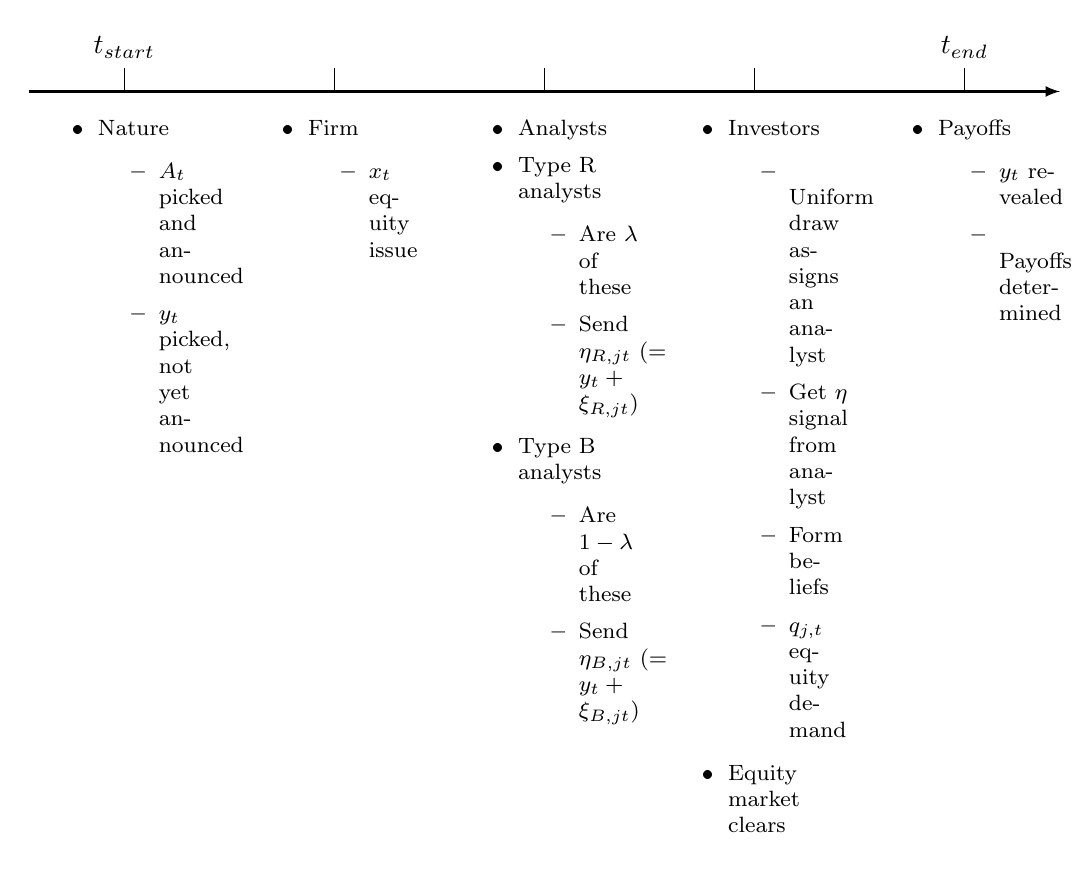
\begin{tikzpicture}[
		node distance = 0mm and 0.02\linewidth,
		box/.style = {inner xsep=0pt, outer sep=0pt,
			text width=0.2\linewidth,
			align=left, font=\footnotesize}
		]
		\node (n1) [box]
		{   \begin{itemize}
				\item Nature
				\begin{itemize}
					\item $A_t$ picked and announced 
					\item $y_t$ picked, not yet announced
				\end{itemize}
			\end{itemize}
		};
		\node (n2) [box, below right=of n1.north east]
		{   \begin{itemize}
				\item Firm 
				\begin{itemize}
					\item $x_t$ equity issue
				\end{itemize}
			\end{itemize}
		};
		
		\node (n3) [box, below right=of n2.north east]
		{   \begin{itemize}
				\item Analysts 
				\item Type R analysts 
				\begin{itemize}
					\item Are $\lambda$ of these
					\item Send $\eta_{R,jt}\ (=y_t +\xi_{R,jt})$
				\end{itemize}
				\item Type B analysts 
				\begin{itemize}
					\item Are $1- \lambda$ of these
					\item Send $\eta_{B,jt}\ (=y_t+\xi_{B,jt})$
				\end{itemize}	
			\end{itemize}
		};
		\node (n4) [box, below right=of n3.north east]
		{   \begin{itemize}
				\item Investors
				\begin{itemize}
					\item Uniform draw assigns an analyst
					\item Get $\eta$ signal from analyst 
					\item Form beliefs
					\item $q_{j,t}$ equity demand
				\end{itemize}
    \item Equity market clears
			\end{itemize}
		};
		\node (n5) [box, below right=of n4.north east]
	{   \begin{itemize}
			\item Payoffs
			\begin{itemize}
				\item $y_{t}$ revealed 
				\item Payoffs determined
			\end{itemize}
		\end{itemize}
	};
	
		\draw[thick, -latex]    (n1.north west) -- (n5.north east);
		\draw (n1.north) -- + (0,3mm) node[above] {$t_{start}$};
		\draw (n2.north) -- + (0,3mm);
		\draw (n3.north) -- + (0,3mm);
		\draw (n4.north) -- + (0,3mm);
		\draw (n5.north) -- + (0,3mm) node[above] {$t_{end}$};
	\end{tikzpicture}
\end{figure}



%%%%%%%%%%%%%%%%%%%%%%%%%%%%%%%%%%%%%%%%%%%%%%%%%%%%%%%
% Tables
%%%%%%%%%%%%%%%%%%%%%%%%%%%%%%%%%%%%%%%%%%%%%%%%%%%%%%%
\clearpage 
\setcounter{table}{0}  
\makeatletter% Set distance from top of page to first float
\setlength{\@fptop}{5pt}
\makeatother


\begin{table}[tbp]
	\caption{Summary Statistics}
	\label{tab:sumstat}
        This table reports the summary statistics of key variables. The mean squared error (MSE) shows the out-of-sample performance of the forecasting models. The MSE for analysts forecasts is 1.315. 
	\begin{center}
        \subcaption{\% ML Win}
        \begin{tabular}{llccc}
        \toprule
        & Forecasting Variables         & Learning rate &  MSE & Ratio   of MSE: Analysts vs ML \\
        \midrule
        (1) & Analysts Forecast &      -      & 1.315 &       -                 \\
        \midrule
        & Gradient Boosting & & &  \\
        \cmidrule(lr){2-2}
        (2) & All                           & 0.1           & 1.261 & 1.043                       \\
        (3) & All minus Analysts Forecast   & 0.1           & 1.506   & 0.873                          \\
        (4) & All plus Financial Statements & 0.1           & 1.258 & 1.045                          \\
        (5) & All                           & 0.01          & 2.582 & 0.509                          \\
        (6) & All                           & 0.4          & 1.289 & 1.020                          \\
        (7) & All                           & 0.5           & 1.322 & 0.995                         \\
        \midrule
        & Random Forest & & &  \\
        \cmidrule(lr){2-2}
        (8) & All                           & -           & 1.278 & 1.029                        \\
        \midrule
        & Neutral Network & Learning Rate& &  \\
        \cmidrule(lr){2-2}
        (9) & All                           & 0.1           & 1.648 & 0.798                        \\
        (10) & All                           & 0.2           & 2.504 & 0.525                        \\
        (11) & All                           & 0.5           & 3.932 & 0.334                        \\
        \midrule
        & Linear Regressions & & &  \\
        \cmidrule(lr){2-2}
        (12) & All                           & -           & 1.779 & 0.739                         \\
          \bottomrule
        \end{tabular}
        \end{center}
\end{table}

\clearpage

%%%%%%%%%%%%%%%%%%%%%%%%%%%%%%%%%%%%%%%%%%%%%%%%%%%%%%%%%%%%%%%%%%%%%%%%

\begin{table}[!ht] %[h!]
	\ContinuedFloat
\caption{Summary Statistics (continued)}
        \begin{center}
        \subcaption{All Analysts}
        \begin{tabular}{lcccccc}
        \toprule
                         & Mean  & Median & Std   Dev & 25     & 75   & N     \\
        \midrule
        EPS               & 1.130 & 0.890 & 1.916 & 0.050 & 1.95 & 54534 \\
        Analyst Forecast  & 1.424 & 1.139 & 1.722 & 0.413 & 2.12 & 54534 \\
        ML Forecast       & 1.151 & 0.884 & 1.508 & 0.199 & 1.82 & 54534 \\
        Analyst Forecast Error & -0.031 & -0.007 & 0.109 & -0.039 & 0.01 & 54534\\
        ML Forecast Error & 0.001 & 0.022 & 0.173 & -0.021 & 0.05 & 54534\\
        Investment        & 0.058 & 0.039 & 0.061 & 0.019  & 0.07 & 54534 \\
        Debt Net Issuance & 0.017 & 0.000 & 0.090 & -0.016 & 0.03 & 54534 \\
        \bottomrule
        \end{tabular}
        \end{center}
       
        \begin{center}
        \subcaption{Tech and Non-Tech Analysts}
        \begin{tabular}{lcccccc}
        \toprule
                         & Mean  & Median & Std   Dev & 25     & 75   & N     \\
        \midrule
        \multicolumn{7}{l}{Sample period: 1994-2018} \\
        EPS                     & 1.351 & 1.06  & 2.168 & 0.11  & 2.28 & 39419 \\
        Non-Tech   Analyst      & 1.678 & 1.341 & 1.996 & 0.483 & 2.5  & 36154 \\
        Tech   Analyst          & 1.669  & 1.198 & 2.442 & 0.253 & 2.65 & 14899 \\
        Non-Tech   Analyst  MSE & 0.837 & 0.027 & 2.981  & 0.003 & 0.2  & 34934 \\
        Tech   Analyst MSE      & 1.604 & 0.039 & 5.723  & 0.005 & 0.34 & 14583 \\
        Investment              & 0.055 & 0.036 & 0.061 & 0.017 & 0.07 & 39773 \\
        \midrule
        \multicolumn{7}{l}{Sample period: 1994-2012} \\
        EPS                     & 1.248 & 1.05  & 1.811 & 0.23  & 2.08 & 25320 \\
        Non-Tech   Analyst      & 1.561 & 1.311 & 1.613 & 0.583 & 2.26 & 22927 \\
        Tech   Analyst          & 1.479 & 1.100   & 1.887 & 0.385 & 2.25 & 7922  \\
        Non-Tech   Analyst  MSE & 0.748 & 0.027 & 2.775 & 0.003 & 0.19 & 22091 \\
        Tech   Analyst MSE      & 1.395 & 0.043 & 5.208  & 0.005 & 0.32 & 7786  \\
        Investment              & 0.06  & 0.039 & 0.064 & 0.02  & 0.07 & 25479 \\
        \midrule
        \multicolumn{7}{l}{Sample period: 2013-2018} \\
        EPS                     & 1.535 & 1.1   & 2.684 & -0.12 & 2.82 & 14099 \\
        Non-Tech   Analyst      & 1.882 & 1.433 & 2.513 & 0.248 & 3.07 & 13227 \\
        Tech   Analyst          & 1.886 & 1.395 & 2.934 & 0.02  & 3.2  & 6977  \\
        Non-Tech   Analyst  MSE & 0.991 & 0.027 & 3.300 & 0.003 & 0.21 & 12843 \\
        Tech   Analyst MSE      & 1.844 & 0.035 & 6.253 & 0.004 & 0.35 & 6797  \\
        Investment              & 0.048 & 0.03  & 0.056 & 0.013 & 0.06 & 14294 \\
        \bottomrule
        \end{tabular}
        \end{center}
\end{table}
\clearpage

%%%%%%%%%%%%%%%%%%%%%%%%%%%%%%%%%%%%%%%%%%%%%%%%%%%%%%%%%%%%%%%%%%%%%%%%

\begin{table}[tbp]
	\caption{Predictable Forecast Errors}
        \label{tab:over_main}
	%\begin{footnotesize}
        This table reports OLS regression results of regressing forecast error at $t+1$ on the information at time $t$. Forecast error at $t+1$ is $\text{Forecast Error}_{t+1} \coloneqq p_{t+1} - F_t p_{t+1} $, where $F_t$ is forecast based on date $t$ data. In columns (1) and (2), forecast $F_t p_{t+1}$ is the average of median monthly earnings forecast of all analysts' forecasts conducted during fiscal year t. In columns (3) and (4), forecast $F_t p_{t+1}$ is the average of median monthly earnings forecast of all machine learning forecasts conducted during fiscal year t. Earnings are converted from EPS forecast to total earnings. Investment$_{t}$ capital expenditure at time $t$. Debt issuance$_{t}$ is net debt issuance at time $t$. All variables are scaled by total assets.
	%\end{footnotesize}	
	\begin{center}
            \begin{tabular}{lcccc}
            \toprule
             & (1)              & (2)              & (3)              & (4)              \\
             & Forecast   Error & Forecast   Error & Forecast   Error & Forecast   Error \\
             & Analysts  &  Analysts   & Machine  & Machine  \\
             \midrule
            Investment& -0.018*   & -0.142*** & -0.018**  & -0.107*** \\
                        & (-1.836)  & (-10.082) & (-2.321)  & (-8.254)  \\
            \midrule
            Firm FE & No        & Yes       & No        & Yes       \\
            Year FE & Yes       & Yes       & Yes       & Yes       \\
            Period  & 1994-2018 & 1994-2018 & 1994-2018 & 1994-2018 \\
            N       & 54541     & 53329     & 54541     & 53329     \\
            AdjR2   & 0.02      & 0.32      & 0.03      & 0.22     \\
            \bottomrule
            \end{tabular}
	\end{center}
\end{table}

\clearpage

%%%%%%%%%%%%%%%%%%%%%%%%%%%%%%%%%%%%%%%%%%%%%%%%%%%%%%%%%%%%%%%%%%%%%%%%
\begin{table}[tbp]
	\caption{Predictable Forecast Errors Using Different Forecasting Variables}
         \label{tab:over_variables}
       % \begin{footnotesize}
         This table presents the results of an OLS regression analysis of the forecast error at time $t + 1$ and Wald test results from seemingly unrelated regressions. The forecast error at $t + 1$ is defined as $\text{Forecast Error}_{t+1} = p_{t+1} - F_t p_{t+1}$, where $F_t p_{t+1}$ is the average of median monthly earnings forecast based on data from time $t$, and $p_{t+1}$ represents the actual earnings at time $t + 1$. Forecasts are calculated from various machine learning models that use different forecasting variables. In column (1), the forecasting variables include firm characteristics. In column (2), the forecasting variables include firm characteristics and analysts forecasts. In column (3), the variables include firm characteristics, analysts forecasts, and financial statement items. All earnings are converted to total earnings from EPS forecasts and scaled by total assets. Investment$_{t}$ is capital expenditure at time $t$. Debt issuance$_{t}$ is net debt issuance at time $t$. The $\chi^2$ of the Wald test is used to test the difference of regression coefficients from column (2), with the results of the test presented in the table. The p-value of the test is also included in brackets.
        %\end{footnotesize}	
	\begin{center}
            \begin{tabular}{lcccc}
            \toprule
             & (1)              & (2)              & (3)               \\
             & Forecast   Error & Forecast   Error & Forecast   Error \\
             & Machine  &  Machine   & Machine   \\
             \midrule
             Investment & -0.111*** & -0.107*** & -0.104*** \\
              & (-7.477)   & (-8.254)  & (-8.107)  \\
             \midrule
             $\chi^2$	 &0.416	& -	&1.718 \\
                    &[0.519]  &-	&[0.182]\\
            Firm FE & Yes              & Yes       & Yes       \\
            Year FE & Yes           & Yes       & Yes       \\
            Forecasting Variables:  &    &    &    \\
            ~~Firm Char. & Yes & Yes & Yes \\
            ~~Analysts Forecasts & No & Yes & Yes \\
            ~~Financial Statement Items& No & No & Yes \\
            Period  & 1994-2018 & 1994-2018 & 1994-2018 \\
            N               & 53329     & 53329     & 53329     \\
            AdjR2         & 0.23      & 0.22      & 0.20     \\
            \midrule
            Forecast MSE  &  1.506 & 1.261 &  1.258\\
            \bottomrule
            \end{tabular}
	\end{center}
\end{table}
\clearpage


%%%%%%%%%%%%%%%%%%%%%%%%%%%%%%%%%%%%%%%%%%%%%%%%%%%%%%%%%%%%%%%%%%%%%%%%


\begin{table}[tbp]
	\caption{Decomposing Forecast Errors }
        \label{tab:over_decompose}
	%\begin{footnotesize}
         This table presents the results of an OLS regression analysis of the forecast error at time $t + 1$.
         We decompose forecast errors into a market-related variation and a firm-specific variation, using the following regression $e_{i,t} = \beta_i + \beta_{i,m} r_{m,t} + \varepsilon_{i,t}$. $e_{i,t}$ is the forecast error of firm $i$ at year $t$, $r_{m,t}$ is the market forecast error at year $t$, which is the equal-weighted average forecast error at year $t$. We define market-related forecast error as $\hat{\beta}_{i,m} r_{m,t}$ and the firm-specific forecast error as $e_{i,t} - \hat{\beta}_{i,m} r_{m,t}$.
         The dependent variable in column (1) is the market-related forecasting errors of human analysts, while column (2) is the firm-specific forecasting errors of human analysts. The dependent variable in column (3) is the market-related forecasting errors of machine analysts, while column (4) is the firm-specific forecasting errors of machine analysts. Investment$_{t}$ is capital expenditure at time $t$.
        %\end{footnotesize}	
	\begin{center}
        \begin{tabular}{lcccc}
            \toprule
             & (1)              & (2)              & (3)              & (4)              \\
             & Forecast   Error & Forecast   Error & Forecast   Error & Forecast   Error \\
             & Analysts  &  Analysts   & Machine  & Machine  \\
             & Market-Related & Firm-Specific & Market-Related & Firm-Specific \\
             \midrule
            Investment& -0.040***     & -0.103***      & -0.012*            & -0.095***            \\
             & (-4.911)      & (-9.381)       & (-1.812)            & (-8.389)             \\
            Firm FE & Yes           & Yes            & Yes                 & Yes                  \\
            Year FE & Yes           & Yes            & Yes                 & Yes                  \\
            Period  & 1994-2018     & 1994-2018      & 1994-2018           & 1994-2018            \\
            N       & 53329         & 53329          & 53329               & 53329                \\
            AdjR2   & 1.00          & 0.99           & 0.99                & 0.96                \\
            \bottomrule
            \end{tabular}
	\end{center}
\end{table}

\clearpage

%%%%%%%%%%%%%%%%%%%%%%%%%%%%%%%%%%%%%%%%%%%%%%%%%%%%%%%%%%%%%%%%%%%%%%%%

\begin{table}[tbp]
\caption{Predictable Forecast Errors Using Different Machine Learning Models}
        \label{tab:over_ml}
	%\begin{footnotesize}
         This table presents the OLS regression results of regressing forecast error at $t + 1$ on the information at time $t$. The forecast error at $t + 1$ is defined as $\text{Forecast Error}_{t+1} = p_{t+1} - F_t p_{t+1}$, where $F_t p_{t+1}$ is the average of monthly earnings forecast based on data from time $t$, and $p_{t+1}$ represents the actual earnings at time $t + 1$. Forecasts are predicted using random forest and neural network algorithms (we use packages from scikit learn to implement the prediction. We have tried a bunch of hyperparameters, and here we only present results with the lowest forecast MSE). In column (1), we use random forest algorithm to make predictions. In column (2), we use neural network algorithm to make predictions. All predictive variables are normalized to be within the range of [0,1] for neural network. Forecast MSE shows the out-of-sample performance of the forecasting model. % (for the sake of space, we only include hyperparameters that use values different from the default)
	\begin{center}
            \begin{tabular}{lcc}
            \toprule
             & (1)              & (2)                \\
             & Forecast   Error & Forecast   Error  \\
             & Random Forest & Neural Network \\
             \midrule
             Investment & -0.129*** & -0.136***\\
             & (-10.078)  & (-6.981)  \\
             \midrule
            Firm FE & Yes        & Yes        \\
            Year FE & Yes        & Yes     \\
            Period  & 1994-2018 & 1994-2018 \\
            N       & 53329        & 53329       \\
            AdjR2   & 0.23          & 0.25     \\
            \midrule 
           Hyperparameters & max\_depth = 5 & learning rate = 0.1  \\
            \midrule 
            Forecast MSE & 1.278 & 1.648 \\
            \bottomrule
            \end{tabular}
            \vspace{3mm}
	\end{center}
\end{table}
\clearpage

%%%%%%%%%%%%%%%%%%%%%%%%%%%%%%%%%%%%%%%%%%%%%%%%%%%%%%%%%%%%%%%%%%%%%%%%

\begin{table}[tbp]
	\caption{Predictable Forecast Errors in Linear Models }
        \label{tab:over_ols}
	%\begin{footnotesize}
         This table presents the results of an OLS regression analysis of the forecast error at time $t + 1$ and Wald test results from seemingly unrelated regressions. The forecast error at $t + 1$ is defined as $\text{Forecast Error}_{t+1} = p_{t+1} - F_t p_{t+1}$, where $F_t p_{t+1}$ is the average of monthly earnings forecast based on data from time $t$, and $p_{t+1}$ represents the actual earnings at time $t + 1$. Forecasts are calculated from linear regression models that use different forecasting variables. In column (1), the forecasting variables include firm characteristics. In column (2), the forecasting variables include firm characteristics and analysts forecasts. In column (3), the variables include firm characteristics, analysts forecasts, and financial statement items. All earnings are converted to total earnings from EPS forecasts and scaled by total assets. Investment$_{t}$ is capital expenditure at time $t$. Debt issuance$_{t}$ is net debt issuance at time $t$. The $\chi^2$ of the Wald test is used to test the difference of regression coefficients from column (3), with the results of the test presented in the table. The p-value of the test is also included in brackets. The mean squared error (MSE) shows the out-of-sample performance of the forecasting models.
       % \end{footnotesize}	
	\begin{center}
            \begin{tabular}{lccc}
            \toprule
             & (1)              & (2)              & (3)                    \\
             & Forecast   Error & Forecast   Error & Forecast   Error \\
             & OLS  &  OLS   & OLS    \\
             \midrule
             Investment  & -0.112*** & -0.084*** & -0.102*** \\
              & (-5.146)   & (-3.962)  & (-5.190)  \\
             \midrule
             $\chi^2$	 &2.225	& 0.096	& 0.084 \\
                   	&[0.136]  & [0.756]	&[0.772]\\
            Firm FE            & Yes       & Yes       & Yes       \\
            Year FE          & Yes       & Yes       & Yes       \\
            Forecasting Variables:   &    &    &    \\
            ~~Firm Char. & Yes & Yes & Yes \\
            ~~Analysts Forecasts & No & Yes & Yes \\
            ~~Financial Statement Items  & No & No & Yes \\
            Period   & 1994-2018 & 1994-2018 & 1994-2018 \\
            N               & 53329     & 53329     & 53329     \\
            AdjR2          & 0.44      & 0.25      & 0.26     \\
            \midrule 
            Forecast MSE& 2.641 & 1.779 & 1.815 \\
            \bottomrule
            \end{tabular}
	\end{center}
\end{table}
\clearpage

%%%%%%%%%%%%%%%%%%%%%%%%%%%%%%%%%%%%%%%%%%%%%%%%%%%%%%%%%%%%%%%%%%%%%%%%

\begin{table}[tbp]
	\caption{Predictable Forecast Errors Using Different Hyper-parameters}
        \label{tab:over_lr}
	%\begin{footnotesize}
         This table presents the results of an OLS regression analysis of the forecast error at time $t + 1$. %and Wald test results from seemingly unrelated regressions
         The forecast error at $t + 1$ is defined as $\text{Forecast Error}_{t+1} = p_{t+1} - F_t p_{t+1}$, where $F_t p_{t+1}$ is the average of median monthly earnings forecast based on data from time $t$, and $p_{t+1}$ represents the actual earnings at time $t + 1$. Forecasts are calculated from machine learning models using different hyper-parameters. The default hyper-parameters and the number of trees in the forest is $50$. Panel (a) reports the results using different learning rates for Gradient Boosting Regression Tree model. Panel (b) reports the results using different learning rates for the Neural Network model. Investment$_{t}$ is capital expenditure at time $t$. The mean squared error (MSE) shows the out-of-sample performance of the forecasting models. % The $\chi^2$ of the Wald test is used to test the difference of regression coefficients from column (3), with the results of the test presented in the table. The p-value of the test is also included in brackets.
        %\end{footnotesize}	
	\begin{center}
        \subcaption{GBRT predictions}
        \begin{tabular}{lcccc}
            \toprule
             & (1)              & (2)              & (3)              & (4)              \\
             & Forecast   Error & Forecast   Error & Forecast   Error & Forecast   Error \\
             & Machine  &  Machine   & Machine  & Machine  \\
             \cmidrule(lr){2-5}
             Learning rate & 0.01  & 0.1 & 0.4 & 0.5 \\
             \midrule
            Investment& 0.028     & -0.107*** & -0.098*** & -0.092** \\
                    & (0.846)   & (-8.254)  & (-6.565) & (-6.065) \\
            \midrule
%            $\chi^2$      & 18.243	& 5.713 & -	&0.428 \\
%            & [0.000]	&[0.017]	 &-	& [0.513]  \\
            Firm FE & Yes       & Yes            & Yes       & Yes       \\
            Year FE & Yes       & Yes             & Yes       & Yes       \\
            Period  & 1994-2018 & 1994-2018  & 1994-2018 & 1994-2018 \\
            N       & 53329     & 53329        & 53329     & 53329     \\
            AdjR2   & 0.76      & 0.22      & 0.18  & 0.18   \\
            \midrule
            Forecast MSE & 2.582& 1.261 & 1.289 & 1.322\\
            \bottomrule
            \end{tabular}
            \subcaption{Neural Network predictions}
            \begin{tabular}{lccc}
            \toprule
             & (1)              & (2)              & (3)           \\
             & Forecast   Error & Forecast   Error & Forecast   Error \\
             & Neural Network  & Neural Network & Neural Network \\
             \midrule
             Investment & -0.136*** & -0.010 & 0.051 \\
              & (-6.981)  & (-0.308) & (1.056) \\
             \midrule
            Firm FE & Yes             & Yes       & Yes       \\
            Year FE & Yes           & Yes       & Yes        \\
            Period  & 1994-2018  & 1994-2018 & 1994-2018  \\
            N       & 53329     & 53329 & 53329    \\
            AdjR2   & 0.25      & 0.36  & 0.72  \\
            \midrule 
           Hyperparameters & learning rate = 0.1 & learning rate = 0.2 & learning rate = 0.5 \\
            \midrule 
            Forecast MSE & 1.648 & 2.504 & 3.932 \\
            \bottomrule
            \end{tabular}
	\end{center}
\end{table}
\clearpage

%%%%%%%%%%%%%%%%%%%%%%%%%%%%%%%%%%%%%%%%%%%%%%%%%%%%%%%%%%%%%%%%%%%%%%%%



\begin{table}[!ht]%[h!]
 \caption{Overreaction test on simulated data}
   This table shows the simulation results. Panel (a) lists all parameter values. The values of parameters are not intended to match data, but serve as an tool to test potential mechanism of overreaction of XGBoost. Panel (b) and (c) display the statistics associated with $\beta$ estimated based on Equation \ref{simu}. Out of the 200 simulated samples, we keep samples with statistically significant $\beta$ (absolute value of t-stat$\geq$1.96). Then we calculate the average $\beta$, average absolute value of forecast errors and MSE averaged across these filtered samples. ``\%significant" is the percentage of $\beta$s with absolute value of t-stat$\geq$1.96. ``\%negative (conditional)" is the percentage of negative $\beta$s conditional on significance. Panel (b) presents the results with positive overreaction. For the 1000 firms in each sample, 66.7\% are set to be consistently rational across all periods, while the rest have time-varying overreaction coefficient $\theta$ which is randomly drawn from uniform distribution $U[0.1,0.3]$. Panel (c) presents the results with no overreaction ($\theta=0$). Learning rate is 0.1.
  \label{tab:simu}  
        \begin{center}
        \subcaption{Parameters}
\begin{tabular}{lcccccc}
        \toprule
       Per share return & $\delta_A$ & $\sigma(\epsilon_A), \rho_A^{-\frac{1}{2}}$ & $\delta$ & $\sigma(\epsilon_z), \rho_y^{-\frac{1}{2}}$ & $\sigma(\eta), \rho_\eta^{-\frac{1}{2}}$ & $\sigma(\tilde x), \rho_x^{-\frac{1}{2}}$\\
       \cmidrule(lr){2-7}
       &  0.10 & 1.00 &  0.60 & 20.00 & 0.80 & 1.00 \\
        \midrule
    Investor decision & $\theta$ & $\lambda$ & $\alpha$ & r & $\mu_y$ & \\
       \cmidrule(lr){2-6}
       &  [0,0.30] & 0.50 & 0.50 & 1.00 & 10.00 & \\
       \midrule
 Firm decision & $\phi$ & & & & & \\
       \cmidrule(lr){2-2}
       &  0.10 & &  & & & \\       
    \bottomrule
        \end{tabular}
        \end{center}
\begin{center}
        \subcaption{Simulation results ($\theta=[0,0.3]$, 66.7\% rational)}
    \begin{tabular}{lcccc}
    \toprule
     & {$\beta$} & {Mean(|fe|)} & {\%significant} & {\%negative}  \\
     &&&&  (conditional)\\
    \cmidrule{2-5}   
    XGBoost  & -0.001 & 16.13 & 17\% & 58\%\\
        OLS  & -0.113 & 62.05 & 72\% & 47\%\\
    \bottomrule
    \end{tabular}%
\end{center}
\begin{center}
        \subcaption{Simulation results ($\theta=0$)}
    \begin{tabular}{lcccc}
    \toprule
    & {$\beta$} & {Mean(|fe|)} & {\%significant} & {\%negative} \\
    &&&&  (conditional)\\
    \cmidrule{2-5}  
    XGBoost & -0.001 & 16.14 & 18\% & 51\% \\
    OLS     & -0.116 & 62.99 & 71\% & 48\% \\
    \bottomrule
    \end{tabular}%
\end{center}
\end{table}
\clearpage

%%%%%%%%%%%%%%%%%%%%%%%%%%%%%%%%%%%%%%%%%%%%%%%%%%%%%%%%%%%%%%%%%%%%%%%%


\begin{table}[tbp]
\caption{Predictable Forecast Errors Using ChatGPT}
        \label{tab:over_gpt}
	%\begin{footnotesize}
         This table presents the OLS regression results of regressing forecast error at $t + 1$ on the information at time $t$. The forecast error at $t + 1$ is defined as $\text{Forecast Error}_{t+1} = p_{t+1} - F_t p_{t+1}$, where $F_t p_{t+1}$ is the average of monthly earnings forecast based on data from time $t$, and $p_{t+1}$ represents the actual earnings at time $t + 1$. The prediction in column (1) is obtained using ChatGPT4o (we directly use this pre-trained model and feed in all the predictors we used for XGBoost baseline results, see Appendix \ref{sec:ai} for the prompt we use). For the sake of computation power and time, we only use the prediction 12 month before the EPS date (instead of taking the median across 12 months' forecasts). To make sure results are comparable, we also include the results from analyst forecasts and XGBoost for the sample sample in columns (2) and (3). All predictive variables are normalized to be within the range of [0,1] for neural network. All earnings are converted to total earnings from EPS forecasts and scaled by total assets. Investment$_{t}$ is capital expenditure at time $t$. Because we directly use the pre-trained ChatGPT model instead of training it, the mean squared error (MSE) shows the in-sample performance of the forecasting models.
	\begin{center}
	\begin{tabular}{lccc}
    \toprule
          & (1)   & (2)   & (3) \\
          & {Forecast Error} & {Forecast Error} & {Forecast Error} \\
          & {ChatGPT} & {Analyst} & {XGBoost} \\
    \midrule
    Investment & {-0.110***} & {-0.164***} & {-0.123***} \\
          & {(-7.165)} & {(-10.173)} & {(-7.846)} \\
    Firm FE & Yes   & Yes   & Yes \\
    Year FE & Yes   & Yes   & Yes \\
    Period & 1994-2018 & 1994-2018 & 1994-2018 \\
    N     & 28002 & 28002 & 28002 \\
    AdjR2 & 0.33  & 0.33  & 0.27 \\
    \midrule 
    Forecast MSE & 1.350 & 1.478 &  1.436 \\
    \bottomrule
	\end{tabular}
	\end{center}
\end{table}
\clearpage

%%%%%%%%%%%%%%%%%%%%%%%%%%%%%%%%%%%%%%%%%%%%%%%%%%%%%%%%%%%%%%%%%%%%%%%%


\begin{table}[tbp]
\caption{Tech Analysts vs Non-Tech Analysts Background before and after 2013}
\label{tab:techinv}
%\begin{footnotesize}
    This table report OLS regression results of regressing forecast error at $t+1$ on the information at time $t$. Forecast error at $t+1$ is $\text{Forecast Error}_{t+1} \coloneqq p_{t+1} - F_t p_{t+1} $, where $F_t$ is forecast based on date $t$ data. In columns (1) and (3), forecast $F_t p_{t+1}$ is the average of median monthly earnings forecast of tech analysts conducted during fiscal year t. In columns (2) and (4), forecast $F_t p_{t+1}$ is the average of median monthly earnings forecast of non-tech analysts conducted during fiscal year t. Earnings are converted from EPS forecast to total earnings. Investment$_{t}$ capital expenditure at time $t$.  All variables are scaled by total assets. Sample periods are reported.
% \end{footnotesize}
    \begin{center}
    \subcaption{Full Sample}\label{tab:techinv_full}
    \begin{tabular}{lcccc}
    \toprule
     & (1)              & (2)              & (3)              & (4)              \\
     & Forecast   Error & Forecast   Error & Forecast   Error & Forecast   Error \\
     & Tech  &  Non-Tech   & Tech  & Non-Tech  \\
     \midrule
    Investment & -0.181*** & -0.127*** & -0.109    & -0.090**  \\
       & (-2.736)  & (-6.922)  & (-1.426)  & (-2.864)  \\
    \midrule
    Firm FE    & Yes       & Yes       & Yes       & Yes       \\
    Year FE    & Yes       & Yes       & Yes       & Yes       \\
    Period     & 1994-2012 & 1994-2012 & 2013-2018 & 2013-2018 \\
    N          & 7367      & 21309     & 6358      & 12316     \\
    AdjR2      & 0.25      & 0.27      & 0.25      & 0.31     \\
    \bottomrule
    \end{tabular}
    \end{center}
    \begin{center}
    \subcaption{Balanced Sample}\label{tab:techinv_bal}
    \begin{tabular}{lcccc}
    \toprule
     & (1)              & (2)              & (3)              & (4)              \\
     & Forecast   Error & Forecast   Error & Forecast   Error & Forecast   Error \\
     & Tech  &  Non-Tech   & Tech  & Non-Tech  \\
     \midrule
    Investment & -0.161**  & -0.119**  & -0.153**  & -0.118**  \\
            & (-2.399)  & (-1.998)  & (-2.365)  & (-2.069)  \\
    \midrule
    Firm FE & Yes       & Yes       & Yes       & Yes       \\
    Year FE & Yes       & Yes       & Yes       & Yes       \\
    Period  & 1994-2012 & 1994-2012 & 2013-2018 & 2013-2018 \\
    N       & 4903      & 4903      & 5100      & 5100      \\
    AdjR2   & 0.25      & 0.26      & 0.29      & 0.32     \\
    \bottomrule
    \end{tabular}
    \end{center}
\end{table}
\clearpage

%%%%%%%%%%%%%%%%%%%%%%%%%%%%%%%%%%%%%%%%%%%%%%%%%%%%%%%%%%%%%%%%%%%%%%%%

\begin{table}[tbp]
\caption{Investment Reversals}
\label{tab:invrev}
%\begin{footnotesize}
    This table reports OLS regression results of regressing changes in investments at $t+1$ and predicted forecast errors. predicted forecast errors. Predicted Forecast Errors (Tech) are predicted value using regression coefficients in Table \ref{tab:techinv} for tech analysts. Predicted Forecast Errors (Non-Tech) are predicted values using regression coefficients in Table \ref{tab:techinv} for non-tech analysts.
%\end{footnotesize}	
    \begin{center}
    \begin{tabular}{lcccc}
    \toprule
     & (1)              & (2)              & (3)              & (4)              \\
     & $\Delta$ Inv$_{t+1}$ & $\Delta$ Inv$_{t+1}$ & $\Delta$ Inv$_{t+1}$ & $\Delta$ Inv$_{t+1}$ \\
     \midrule
    Predicted Forecast  & 6.527***  &           & 4.557***   &           \\
    Errors (Tech)     & (5.118)  &           & (2.861)   &           \\
    Predicted Forecast  &           & 6.131***  &           & 5.374***  \\
    Errors (Non-Tech)  &           & (4.555)   &           & (5.459)   \\
    \midrule
    Firm FE & Yes       & Yes       & Yes       & Yes       \\
    Year FE & Yes       & Yes       & Yes       & Yes       \\
    Period  & 1994-2012 & 1994-2012 & 2013-2018 & 2013-2018 \\
    N       & 54        & 163       & 187       & 349       \\
    AdjR2   & 0.29      & 0.41      & 0.09     & 0.11     \\
        \bottomrule
    \end{tabular}
    \end{center}
\end{table}
\clearpage

%%%%%%%%%%%%%%%%%%%%%%%%%%%%%%%%%%%%%%%%%%%%%%%%%%%%%%%%%%%%%%%%%%%%%%%%


\begin{table}[tbp]
    \caption{Tech Analyst Coverage}
    \label{tab:techcoverage}
 %   \begin{footnotesize}
        This table estimates average characteristics of the stocks that tech analysts at analyst-year level. Tech is a indicator variables equalling to 1 if the analyst is tech analyst, 0 otherwise. After 2013 is an indicator variable equaling to 1 if the forecast is made after 2013. Number of Stocks is the total number of stocks covered by the analyst. Age is the average age of the stocks covered by the analyst. Total assets is the average total assets of stocks covered by the analyst. High Tech is the percentage of high-tech stocks covered by the analyst. High-Tech stocks are firms with three digit SIC code of 283, 357, 366, 367, 382, 384, or 737.
 %   \end{footnotesize}	
%    \subcaption{Coverage before and after 2013}
    \begin{center}
    \subcaption{Coverage before and after 2013}
    \begin{tabular}{lcccc}
    \toprule
     & (1)              & (2)              & (3)              & (4)              \\
     & Num of Stocks & Age       & Total   Assets & High Tech \\
    \midrule
    Tech*After 2013 & 0.839***          & -0.223    & -0.019         & -0.002      \\
                    & (2.963)           & (-0.891)  & (-0.586)       & (-0.381)    \\
    \midrule
    Analyst FE      & Yes               & Yes       & Yes            & Yes         \\
    Year FE         & Yes               & Yes       & Yes            & Yes         \\
    Period          & 1994-2018         & 1994-2018 & 1994-2018      & 1994-2018   \\
    N               & 11703             & 11703     & 11703          & 11703       \\
    AdjR2           & 0.57              & 0.77      & 0.79           & 0.92       \\
    \bottomrule
    \end{tabular}
    \end{center}
    %\subcaption{Tech Analysts Coverage}
    \begin{center}
    \subcaption{Tech Analysts Coverage}
    \begin{tabular}{lcccc}
    \toprule
     & (1)     & (2)     & (3)    & (4)     \\
     & Num of Stocks & Age    & Total Assets & High Tech \\
    \midrule
    Tech       & -0.048    & -1.690*** & -0.194*** & 0.220***  \\
           & (-0.256)  & (-7.374)  & (-6.299)  & (22.984)  \\
    \midrule
    Analyst FE & No        & No        & No        & No        \\
    Year FE    & Yes       & Yes       & Yes       & Yes       \\
    Period     & 1994-2018 & 1994-2018 & 1994-2018 & 1994-2018 \\
    N          & 11716     & 11716     & 11716     & 11716     \\
    AdjR2      & 0.06      & 0.06      & 0.06      & 0.04     \\
    \bottomrule
    \end{tabular}
    \end{center}
\end{table}
\clearpage

%%%%%%%%%%%%%%%%%%%%%%%%%%%%%%%%%%%%%%%%%%%%%%%%%%%
\appendix
\section{Appendix}
\setcounter{table}{0}
\renewcommand{\thetable}{A\arabic{table}}
\clearpage
\begin{table}[tbp]
\caption{Technical Majors }
\label{tab:majors}\vspace{2 mm}
\par
\centering
\begin{tabular}{ll}
\toprule
Transportation                        & Finance, Physics                          \\
Systems engineering                   & Finance, IT                               \\
Quantitative Econ, Financial Modeling & Finance and Information Syatems           \\
quantitative analysis                 & Environmental Engineering                 \\
Quantatitive finance                  & Engineering                               \\
Quant econ course                     & Eletrical, Ocean, Civil Engineering       \\
Physics and Economics                 & Eletrical Engineering, CS                 \\
Physics and applied math              & Electronics and communication enginerring \\
Physics                               & Electrical engineering                    \\
PhD Pharmaceutical sciences           & Electrical Electronic Engineering         \\
PhD in Pharmacology                   & Electrical Computer Engineering           \\
PhD in neuroscience                   & Electrical and electronics engineering    \\
PhD Biomedical/Medical Engineering    & Data analyst course                       \\
Computer                              & Computer Science                          \\
Mehcanical Engineering                & Computer engineering                      \\
Medical Chemistry                     & Computer engineering                      \\
Mechanical Engineering                & Computational biology, bioinformatics     \\
Mathematics, Finance                  & Computatioanl finance, information system \\
Mathematics, economics                & Civil Engineering                         \\
Mathematics, acturial studies         & Civil engineering                         \\
Mathematics minor                     & Chemistry, environmental engineering      \\
Mathematics and statistics            & Chemistry engineering                     \\
Mathematics and physics               & Chemistry and Applied mathematics         \\
Mathematics                           & Chemistry                                 \\
Mathematical science                  & Chemical Engineering                      \\
Mathematical economics analysis       & Biophysics and biochemistry               \\
Mathematical economics                & biophysics                                \\
Mathematic, Physics                   & Bio-Organic Chemistry                     \\
Mathematic and economics              & biomedical engineering                    \\
Math and Economics                    & BioMathematics                            \\
Materials Science                     & Biology and chemistry                     \\
Material metallurgical engineering    & Biology and Biochemistry                  \\
Masters in Data Science               & Biochemistry                              \\
Master of engineering                 & behavioral science                        \\
M.A. in Neuroscience                  & Information systems                       \\
Industrial Engineering                &                                           \\
Industrial and system engineering     &                                           \\
Industrial and management engineering &                                           \\
general engineering                   &                                           \\
Financial Modeling, Engineering       &                             \\   
\bottomrule
\end{tabular}
\end{table}
\clearpage


\begin{table}[tbp]
	\caption{Predictable Forecast Errors}
 \label{tab:over_gmm}
	\begin{footnotesize}      
        This table report GMM regression results of regressing forecast error at $t+1$ on the information at time $t$. Forecast error at $t+1$ is $\text{Forecast Error}_{t+1} \coloneqq p_{t+1} - E_t p_{t+1} $, where $E_t$ is forecast based on date $t$ data. In columns (1), forecast $E_t p_{t+1}$ is the median earnings forecast of all analysts forecasts conducted during fiscal year t. In columns (3), forecast $E_t p_{t+1}$ is the median earnings forecast of all machine learning forecasts conducted during fiscal year t. Earnings are converted from EPS forecast to total earnings. Investment$_{t}$ capital expenditure at time $t$. Debt issuance$_{t}$ is net debt issuance at time $t$. All variables are scaled by total assets.
	\end{footnotesize}	
	\begin{center}
            \begin{tabular}{lcccc}
            \toprule
             & (1)              & (2)                   \\
             & Forecast   Error & Forecast   Error  \\
             & Analysts   & Machine  \\
             \midrule
            Investment&     -0.472***   & -0.345** \\
                          & (0.003)   & (0.025)  \\
            \midrule
            Firm FE & Yes        & Yes           \\
            Year FE & Yes       & Yes            \\
            Period  & 1994-2018 & 1994-2018  \\
            N       & 54536     & 53324      \\
            \bottomrule
            \end{tabular}
	\end{center}
\end{table}
\clearpage

\begin{table}[tbp]
	\caption{Predictable Forecast Errors Using Large Learning Rates}
        \label{tab:largelr}
	\begin{footnotesize}    
         This table presents the results of an OLS regression analysis of the forecast error at time $t + 1$ and Wald test results from seemingly unrelated regressions. The forecast error at $t + 1$ is defined as $\text{Forecast Error}_{t+1} = p_{t+1} - F_t p_{t+1}$, where $F_t p_{t+1}$ is the average of median monthly earnings forecast based on data from time $t$, and $p_{t+1}$ represents the actual earnings at time $t + 1$. Forecasts are calculated from various machine learning models that use different hyper-parameters. The default hyper-parameters are set as the following values: depth of the tree is $2$ and number of
        trees in the forest is $50$. Table reports the results using different learning rates. Investment$_{t}$ is capital expenditure at time $t$. The $\chi^2$ of the Wald test is used to test the difference of regression coefficients from default hyper parameters, with the results of the test presented in the table. The p-value of the test is also included in brackets.
        \end{footnotesize}	
	\begin{center}
        \begin{tabular}{lcccc}
            \toprule
             & (1)              & (2)              & (3)              & (4)              \\
             & Forecast   Error & Forecast   Error & Forecast   Error & Forecast   Error \\
             & Analysts  &  Analysts   & Machine  & Machine  \\
             \cmidrule(lr){2-5}
             Learning rate & 0.15 & 0.25  & 0.3 & 0.5 \\
             \midrule
            Investment& -0.106***       & -0.107***       & -0.105***       & -0.099***       \\
                & (-7.766)        & (-7.285)        & (-7.262)        & (-6.132)        \\
                \midrule
            $\chi^2$      & 0.019	&0.012	 & 0.072&1.261  \\
            & [0.890]	&[0.911]	 &[0.788]	& [0.261]  \\
            Firm FE & Yes             & Yes             & Yes             & Yes             \\
            Year FE & Yes             & Yes             & Yes             & Yes             \\
            Period  & 1994-2018       & 1994-2018       & 1994-2018       & 1994-2018       \\
            N       & 53321           & 53321           & 53321           & 53321           \\
            AdjR2   & 0.21            & 0.20            & 0.20            & 0.18           \\
            \bottomrule
            \end{tabular}
	\end{center}
\end{table}
\clearpage


\begin{table}[tbp]
	\caption{Analysts Forecast Errors}
 \label{tab:analystsinvestment}
	\begin{footnotesize}      
        This table report OLS regression regressing firm investment and debt on analysts forecast errors.
	\end{footnotesize}	
	\begin{center}
            \begin{tabular}{lcccc}
            \toprule
             & (1)       & (2)       & (3)             & (4)             \\
             & Inv$_{t+1}$   & Inv$_{t+1}$   & Debt Net Iss.$_{t+1}$ & Debt Iss.$_{t+1}$ \\
             \midrule
            Analysts Forecast Errors & -0.007*** & -0.007*** & -0.028***       & -0.032***       \\
                         & (-2.668)  & (-3.446)  & (-6.466)        & (-6.017)        \\
                         &           &           &                 &                 \\
            Profit & 0.035***  & 0.020***  & -0.001          & 0.017***        \\
                         & (10.683)  & (6.617)   & (-0.323)        & (4.174)         \\
            Firm FE      & No        & Yes       & No              & Yes             \\
            Year FE      & Yes       & Yes       & Yes             & Yes             \\
            Period       & 1994-2018 & 1994-2018 & 1994-2018       & 1994-2018       \\
            N            & 64218     & 62788     & 64218           & 62788           \\
            AdjR2        & 0.05      & 0.65      & 0.02            & 0.07   \\
            \bottomrule
            \end{tabular}
	\end{center}
\end{table}
\clearpage


\end{document} 



\subsection{Predictable Forecast Errors}\label{sec:framework}
In this section, we present a simple model of predictable forecast errors to clarify the overreaction tests and the sources of forecasting errors. We analyze how machine learning algorithm may improve the predictive power, and how future forecast errors could be correlated with historical information.

Assume analysts or Machine predicts the the value of EPS $y_{i,t}$ for firm $i$ in period $t$. $y_{i,t}$ follows the following process
\begin{equation}
    y_{i,t+1} = \delta y_{i,t} + f(z_{i,t})  + \varepsilon_{i,t+1}\label{process}
\end{equation}
where $f(z_{i,t})$ can be interpreted as firm/type specific component, but determined by information at time $t$. And the forecast is
\begin{equation}
    F_t y_{i,t+1} = \hat{\delta} y_{i,t} + \hat{f}(z_{i,t}) + \theta\hat\delta\varepsilon_{i,t},
\end{equation}
where $\theta>0$ captures the behavioral bias as in \cite{bordalo2021real}.

%The MSE of the forecast is then
%\begin{align}
 %   E(y_{i,t+1} - F_t y_{i,t+1})^2
 %   & =E((\delta - \hat{\delta})y_{i,t} + ( f(z_{i,t}) - \hat{f}(z_{i,t})) - \theta \hat\delta\varepsilon_{i,t} + \varepsilon_{i,t+1})^2 \label{s12}\\
%    & = (\delta - \hat{\delta})^2 E(y_{i,t})^2 + E( f(z_{i,t}) - \hat{f}(z_{i,t}))^2 + \theta^2\hat\delta^2 E(\varepsilon_{i,t})^2 + E(\varepsilon_{i,t+1})^2 \label{s22}.
%\end{align}
%Notice that to go from Equation \ref{s12} to Equation \ref{s22}, it is assumed that all four components in Equation \ref{s12} are uncorrelated with each other.

Without loss of generality assume that $\delta = \hat{\delta}$. Forecast Error is then
\begin{align}
    fe_{i,t+1} & \equiv y_{i,t+1} - E_t y_{i,t+1}  =  \delta y_{i,t} + f(z_{i,t})  + \varepsilon_{i,t+1} - (\hat{\delta} y_{i,t} + \hat{f}(z_{i,t})) - \theta\hat\delta \varepsilon_{i,t}  \\
    & = (\delta - \hat{\delta})y_{i,t} - ( f(z_{i,t}) - \hat{f}(z_{i,t})) - \theta\hat\delta \varepsilon_{i,t}\\
    & =  - \theta \hat\delta\varepsilon_{i,t} - ( f(z_{i,t}) - \hat{f}(z_{i,t}))\label{ferror}
\end{align}

Let $x_{i,t}$ be the observed firm fundamental (e.g., investment) that is linearly related to the forecasted variable $x_{i,t} = \alpha y_{i,t} + \epsilon^x_{i,t}$. We calculate the correlation between investment and forecast errors instead of using lagged earnings and forecast errors in order to address the potential measurement errors in EPS that could potentially affect our analysis (\citet{bordalo2021real}). Calculating the correlation between future forecast errors and current period information, we have
\begin{align}
    cov & (fe_{i,t+1},x_{i,t})  =
     cov( - \theta \hat\delta\varepsilon_{i,t} - ( f(z_{i,t}) - \hat{f}(z_{i,t})) , \alpha \varepsilon_{i,t} ) \label{s2} \\
    & = - \alpha\theta\hat\delta var(\varepsilon_{i,t})\label{s3}.
\end{align}
To get the Equation \ref{s2}, we assume that $f(z_{i,t})-\hat f(z_{i,t})$ is uncorrelated with information prior to time $t$. Equation \ref{s3} says when predictors exhibit behavioral bias ($\theta>0$), forecast error is negatively related to current information $x_{it}$.

With the existence of firm-level heterogeneity, machine learning could improve predictive power by allowing more factors and more complex functional forms. In this setting, we can still utilize the correlation between forecast errors and firm fundamentals to test forecast overreaction. Furthermore, this calculation demonstrates that disregarding firm-level heterogeneity $f(z_{it})$ does not impact the extent of overreaction. The analysis implies that even though machine learning models may produce improved forecasts (i.e., lower mean squared error), it does not necessarily imply that machine learning forecasts exhibit less overreaction.
